\documentclass{article}


% if you need to pass options to natbib, use, e.g.:
%     \PassOptionsToPackage{numbers, compress}{natbib}
% before loading neurips_2025


% ready for submission
% \usepackage{neurips_2025}
% \usepackage[preprint]{neurips_2025}
\usepackage[final]{neurips_2025}



% to avoid loading the natbib package, add option nonatbib:
%    \usepackage[nonatbib]{neurips_2025}
\renewcommand{\paragraph}[1]{\noindent \textbf{#1}}
% other macros
\newcommand{\hanna}[1]{\textcolor{purple}{[Hanna]: #1}}

\usepackage[colorlinks=true, urlcolor={blue!70!black}, linkcolor={blue!70!black}, citecolor={blue!70!black}, pdfborder={0 0 0}]{hyperref}

\usepackage[utf8]{inputenc} % allow utf-8 input
\usepackage[T1]{fontenc}    % use 8-bit T1 fonts
% \usepackage{hyperref}       % hyperlinks
\usepackage{hyperref}
\usepackage{url}            % simple URL typesetting
\usepackage{booktabs}       % professional-quality tables
\usepackage{amsfonts}       % blackboard math symbols
\usepackage{nicefrac}       % compact symbols for 1/2, etc.
\usepackage{microtype}      % microtypography
% \usepackage{xcolor}         % colors

\bibpunct{(}{)}{;}{a}{,}{,}

\usepackage{amsmath}
\usepackage{amsthm}
\usepackage{mathtools}
\usepackage{cleveref}
\usepackage{thm-restate}
\usepackage{paralist}

\usepackage[dvipsnames]{xcolor}
\usepackage[most]{tcolorbox}

% Draft comments.
\newcommand\WM[1]{\textsf{\textcolor{orange}{WM: #1}}}
\newcommand\DG[1]{\textsf{\textcolor{blue}{DG: #1}}}
\newcommand\SA[1]{\textsf{\textcolor{purple}{SA: #1}}}

% Norms and absolute value.
\DeclarePairedDelimiter\abs{\lvert}{\rvert}%
\DeclarePairedDelimiter\norm{\lVert}{\rVert}%

\newtheorem{proposition}{Proposition}

% Box for methods.
\tcbset{
  method/.style={
    colback=RoyalBlue!5,    % Background color
    colframe=RoyalBlue!80,  % Border color
    coltitle=white,    % Title color
    fonttitle=\bfseries,
    boxrule=0.5pt,     % Border thickness
    arc=2mm,           % Rounded corners
    left=6pt,
    right=6pt,
    top=6pt,
    bottom=6pt,
    enhanced,
    sharp corners=south, % flat bottom
    title={Method}   % Default title (can be overridden)
  }
}

% Define the environment using the style, with a counter and title support
% \newtcolorbox[auto counter]{methodbox}[2][]{%
%   method,
%   title={Method~\thetcbcounter: {\hypersetup{citecolor=white} #2}},
% }
\newtcolorbox{methodbox}[2][]{%
  method,
  title={{\hypersetup{citecolor=white} #2}},
}
\crefname{methodbox}{method}{methods}
\Crefname{methodbox}{Method}{Methods}

% Box for assumptions.
\tcbset{
  assumption/.style={
    colback=Maroon!5,    % Background color
    colframe=Maroon!80,  % Border color
    coltitle=white,    % Title color
    fonttitle=\bfseries,
    boxrule=0.5pt,     % Border thickness
    arc=2mm,           % Rounded corners
    left=6pt,
    right=6pt,
    top=6pt,
    bottom=6pt,
    enhanced,
    sharp corners=south, % flat bottom
    title={Assumption}   % Default title (can be overridden)
  }
}

% Define the environment using the style, with a counter and title support
\newtcolorbox[auto counter]{assumptionbox}[2][]{%
  assumption,
  title={Assumption~\thetcbcounter: {\hypersetup{citecolor=white} #2}},
}

\newcommand\Bbig{B_\mathrm{big}}
\newcommand\Bsmall{B_\mathrm{small}}
\newcommand\nGbig{\norm{G_\mathrm{big}}^2}
\newcommand\nGsmall{\norm{G_\mathrm{small}}^2}

\newcommand\upd[1]{{\color{orange} #1}}
\renewcommand\upd[1]{#1}  % Uncomment for CR

\title{Critical Batch Size Revisited: A Simple Empirical Approach to Large-Batch Language Model Training}

% The \author macro works with any number of authors. There are two commands
% used to separate the names and addresses of multiple authors: \And and \AND.
%
% Using \And between authors leaves it to LaTeX to determine where to break the
% lines. Using \AND forces a line break at that point. So, if LaTeX puts 3 of 4
% authors names on the first line, and the last on the second line, try using
% \AND instead of \And before the third author name.


% TODO: add affiliations
\author{%
  William Merrill \quad
  % \texttt{willm@allenai.org} \\
  % \And
  Shane Arora \quad
  % \texttt{shanes@allenai.org} \\
  % \And
  Dirk Groeneveld \quad
  % \texttt{dirkg@allenai.org} \\
  % \And
  Hannaneh Hajishirzi \\
  % \texttt{hannah@allenai.org} \\
  Allen Institute for AI \\
  % Seattle, WA, USA \\
  \texttt{willm@allenai.org}
  % \texttt{\{willm,shanes,dirkg,hannah\}@allenai.org}
}


\begin{document}

\maketitle


\begin{abstract}
    The right batch size is important when training language models at scale: a large batch size is necessary for fast training, but a batch size that is \emph{too large} will harm token efficiency. To navigate this tradeoff, \citet{mccandlish2018empirical} suggest that a \emph{critical batch size} (CBS), below which training will not substantially degrade loss, can be estimated based on the gradient noise scale during training. While their method has been adopted in practice, e.g., when training GPT-3, strong assumptions are required to justify gradient noise as a proxy for the CBS, which makes it unclear whether their approach should be trusted in practice, limiting its applicability. In this paper, we introduce a simple, empirical approach to \emph{directly} measure the CBS and show how the CBS evolves over training. Applying our approach to the OLMo models, we find that CBS is near 0 at initialization, increases rapidly at first, and then plateaus as training progresses. Furthermore, we find that this trend holds across different model sizes (1B and 7B), suggesting CBS from small training runs can inform larger-scale training runs. Our findings about how the CBS changes over training motivate \emph{batch size warmup} as a natural way to reliably train language models at large batch size: start the batch size small and increase it as the CBS grows. To validate this claim, we use batch size warmup to train OLMo 1B to slightly better loss than the original training run with 43\% fewer gradient steps. This shows how our framework can be applied to reliably train language models at larger batch sizes, increasing data parallelism without compromising performance.
\end{abstract}


\section{Introduction}

Increasing the throughput of training is important for training large models.
A natural way to increase throughput is by increasing data parallelism, i.e., increasing the \emph{batch size} used during training so that more data can be processed at once and the number of sequential gradient steps can be decreased.
% With multi-GPU training, a major bottleneck in training speed is the communication overhead between GPUs when taking a gradient step.
% Thus, a natural way to increase token efficiency is to reduce the number of gradient steps that need to be made by \emph{increasing the batch size}.
However, naively picking a very large batch size can degrade the performance achieved by a fixed token budget, as larger batches can show diminishing returns in their ability to estimate the population gradient.
Thus, in order to confidently train language models with higher token throughput, it is important to develop theoretical and empirical understanding of large-batch training.

One fundamental concept for large-batch training methodology is the following:

\begin{methodbox}{Critical Batch Size Hypothesis \citep{mccandlish2018empirical}}
There is some critical batch size $B^*$ up to which increasing the batch size (and appropriately modifying the  learning rate) approximately preserves the loss trajectory as a function of tokens trained, but, above which, the loss trajectory degrades.
\end{methodbox}

If such a CBS $B^*$ exists (and we can measure it), it represents a reasonable balance between efficiency and performance (i.e., loss) and is thus a practically useful batch size at which to train.
Working in a simplified theoretical setup, \citet{mccandlish2018empirical} derive a correspondence between the CBS and the \emph{gradient noise scale}, i.e., the variance of the per-example gradients from the training distribution.
They suggest that an estimator for the gradient noise scale should be used in practice as a proxy for the CBS, and this can in turn be used to set the batch size for large-scale pretraining runs.
The noise scale also appears to have been adopted in practice as a proxy for the CBS, having been mentioned explicitly in the GPT-3 technical report \citep{brown2020language}, and inspiring a flurry of methodological innovations for better noise scale estimation \citep{gray2023efficient,gray2024normalization}.

While appealing, the link between the gradient noise and the CBS requires several strong assumptions to justify: specifically, it assumes the SGD optimizer and that gradients are well-conditioned (cf.~\Cref{sec:noise-scale}).
Thus, it is unclear whether the noise scale should be a meaningful proxy for the CBS for language model pretraining in practice, where the Adam optimizer is often used and the optimization may not be well-conditioned.
To this end, we aim to address the following practical questions that remain for effectively leveraging the CBS viewpoint to train language models at larger batch sizes:

\begin{enumerate}
    \item How can we measure the CBS cheaply with minimal assumptions before launching a pretraining run?
    \item How does the CBS change over the course of pretraining and as a function of model size? 
    \item Having measured the CBS, how should we adapt the batch size, learning rate, and other parameters over the course of a pretraining run?
\end{enumerate}

This work documents our attempts to answer these questions in order to operationalize the CBS for large-batch training.
We focus our investigation on the OLMo models \citep{groeneveld-etal-2024-olmo,olmo20252olmo2furious}, due to their open weights and data, making the following contributions:

\begin{enumerate}
    \item First, we introduc an empirical method to directly measure the CBS via \textbf{branched training}. Our method avoids strong assumptions needed to justify the noise scale method from prior work. This lets us trust it more than the noise scale method, which we find unreliable.
    \item We use our method to study how our CBS measurement changes over the course of training, finding it improves rapidly initially but than flattens off. Further, we find that the CBS not depend strongly on model size, in line with past findings using different methodology \citep{zhang2024cbs}.
    \item Our knowledge of the local CBS across training checkpoints suggest a natural \textbf{batch size warmup} strategy for large batch training: begin training with a small batch size and double it whenever the CBS increases sufficiency. We use this strategy to train 1B parameter models with 43\% fewer gradient steps without degrading (and, in fact, slightly improving) final loss.
\end{enumerate}
Overall, our empirical framework for measuring and leveraging the CBS provides simple and principled methodology for improving the efficiency of large-scale training runs and addressing other fundamental questions in the science of language model pretraining.

% \WM{Lots more prior work to cite. See related work section here: \url{https://arxiv.org/pdf/2410.21676}}

\section{Background: Estimating CBS via Gradient Noise Scale} 
\label{sec:noise-scale}

Past empirical work has aimed to measure the CBS by 
launching many training runs to the same target loss, which is expensive \citep{zhang-2019-algorithmic,zhang2024cbs},
or by using the gradient noise scale as a proxy \citep{mccandlish2018empirical,gray2023efficient,gray2024normalization}. 
In contrast, we will introduce a new method that uses a small amount of additional training to estimate the CBS, which is less expensive than launching many full training runs and does not make any strong assumptions like the noise scale.
Before introducing our method, we review the noise scale framework used to estimate the CBS in prior work and the underlying assumptions it relies on.

\citet{mccandlish2018empirical} suggest that the CBS can be measured in terms of the gradient noise scale, i.e., the variance of the gradients within a batch.
Concretely, their recommendations to measure the CBS and adapt the learning rate are as follows:

\begin{methodbox}{Existing Method: Noise Scale Proxy for CBS \citep{mccandlish2018empirical}}
    Let $G$ be the full gradient and let $\Sigma$ be the covariance matrix for the gradient across data examples.
    We first compute $\mathcal B_\mathsf{simple}$ as a proxy for the CBS (using an efficient statistical estimator):
    \begin{equation*}
        \mathcal B_\mathsf{simple} = \frac{\mathrm{tr}(\Sigma)}{\norm{G}^2} . \label{eq:noise-scale}
    \end{equation*}
    We set the modified batch size to $\mathcal B_\mathsf{simple}$ and \emph{linearly} scale the learning rate $\eta^*$:
    \begin{align}
        B^* &= \mathcal B_\mathsf{simple} \\
        \eta^* &= \frac{B^*}{B} \cdot \eta . \label{eq:linear-scaling}
    \end{align}
\end{methodbox}

This viewpoint is attractive due to its simplicity and tractability, and it has inspired improved methods for estimating the noise scale \citep{gray2023efficient,gray2024normalization}.
However, the link between noise scale and CBS requires several strong assumptions to justify, which we will argue motivates revisiting other approaches for measuring the CBS.
\citet{mccandlish2018empirical} consider training a model on a loss surface where the loss landscape is well approximated by its second-order Taylor expansion.
The first crucial assumption in their analysis is that optimizer used to decrease the loss is SGD:

\begin{assumptionbox}{SGD Optimizer \citep{mccandlish2018empirical}}
    The step taken to reduce the loss is a noisy estimate of the true gradient, computed via $B$ samples.
\end{assumptionbox}

This assumption may seem benign, but it is worth noting that it is \emph{not} typically met in practice, as LMs are trained with the Adam optimizer \citep{kingma-2017-adam}.
Moreover, by analyzing training dynamics in terms of stochastic differential equations \citep{li2021validity}, \citet{malladi2022sdes} argue theoretically that \Cref{eq:linear-scaling} is an appropriate scaling rule for SGD, but not for Adam, where a \emph{square-root} scaling rule is more principled.
\upd{The square-root scaling for Adam is also supported by the theoretical analysis of \citet[Equation 4]{li2024surge}.
Thus, when training with Adam, it seems that the linear scaling rule assumed by \citet{mccandlish2018empirical} should not apply.}
% is unclear whether the noise scale should be a valid proxy for CBS, and, if so, how to operationalize the scaling rule for learning rate.

A more fundamental issue is that \citet{mccandlish2018empirical} also require another strong assumption to derive the noise scale method for estimating the CBS.
In general, their noise-scale-based estimate of the CBS has a more complex form than $\mathcal B_\mathrm{simple}$ involving the Hessian $H$:
\begin{equation*}
    \mathcal B_\mathrm{noise} = \frac{\mathrm{tr}(\Sigma H)}{G^\top H G} .
\end{equation*}
In order to justify that $B^*$ can be computed as $\mathcal B_\mathrm{simple}$,
\citet{mccandlish2018empirical} assume:

\begin{assumptionbox}{Well-Conditioned Optimization \citep{mccandlish2018empirical}}
    The Hessian $H$ is a multiple of the identity matrix. It follows that $\mathcal B_\mathrm{noise} = \mathcal B_\mathrm{simple}$.
\end{assumptionbox}

This is a strong assumption required to justify using $\mathcal B_\mathrm{simple}$ as a proxy for the CBS because computing Hessians would be too expensive to be practice.
\citet{mccandlish2018empirical} suggest informally that, without this assumption, $\mathcal B_\mathrm{simple}$ \emph{may} still be correlated with $\mathcal B_\mathrm{noise}$, but it is not obvious why this should be the case.
Even if this is true, it still poses a real problem for the noise scale methodology, since the goal of the method is to produce an \emph{absolute} measure of $B^*$. It is unclear for practitioners what coefficient should be used to translate $\mathcal B_\mathrm{simple}$ to $B^*$---and, more fundamentally, whether it is even valid to assume that such a coefficient exists.

\section{Our Method: Measuring the CBS via Local Branched Training} \label{sec:our-method}

As discussed in \Cref{sec:noise-scale}, using the gradient noise scale $\mathcal B_\textrm{simple}$ as a proxy to estimate the CBS relies on several strong assumptions.
In light of this, it unclear whether we can trust the gradient noise scale as a proxy for CBS.
We thus argue that we should instead aim to measure the CBS \emph{directly}, without the need for any strong assumptions to justify an indirect proxy.
After introducing our measurement approach in this section, we will show in \Cref{sec:batch-size-warmup} how these measurements can be applied to train language models to the same (or better) target loss with fewer gradients steps.
% \hanna{one big question that arises is: why has nobody done this before if we call this method "simple" and we can calculate things directly? I feel like we are underselling the contribution or observation here?}

\subsection{Method}

We introduce a simple \textbf{branched training} method that directly approximates the CBS by launched branched training runs from a checkpoint, which allows us to identify $B^*$ as the largest batch size that does not degrade in loss relative to smaller batch sizes as visualized in \Cref{fig:measure-cbs}. 
To make this tractable, we train only for a fixed token budget $\Delta$, assuming that if $B^*$ recovers in loss by $\Delta$, its loss will continue to match smaller batch sizes onwards as well.
This allows us to estimate the CBS with only a small amount of additional training (controlled by $\Delta$). 
Further, as we will find later in \Cref{fig:measure-cbs}, the CBS trend remains consistent across model sizes, so CBS measurements with small models could be used to inform large-scale training runs.

% \hanna{another idea, can we show it with a figure? like show the delta sliding windoes and somehow show the max k, etc. } \WM{That was my intent with \Cref{fig:loss-curves}, but maybe I can change it to make the full method clearer}
% \hanna{sounds good... can you refer to figure 1 then in the above description? }


\begin{methodbox}{Our Method: Branched Training to Measure CBS} \label{box:empirical-cbs}
    Given a training checkpoint with original batch size $B$ and learning rate schedule $\eta$, we aim to measure the critical batch size $B^*$.
    Let $f(\eta)$ be the learning rate scaling rule: $f(k) = k$ for SGD and $\sqrt{k}$ for Adam.
    We create several training branches with modified batch size $k \cdot B$ and learning rate $f(k) \cdot \eta$ and train for a small number of tokens $\Delta$ to get loss $L_k$---following standard practice, we take $L_k$ to be the smoothed loss.
    We then define $k^*$ as the maximum $k$ such that, for all $k < k^*$, $L_{k^*} \leq L_k + \epsilon$, where $\epsilon$ is a tolerance parameter for ``similar'' losses.
    
    \paragraph{} We  then define the CBS $B^*$ and scaled learning rate $\eta^*$ as
    \begin{align*}
        B^* &= k^* \cdot B \\
        \eta^* &= f(k^*) \cdot \eta .
    \end{align*}
\end{methodbox}

\begin{figure}
    \centering
    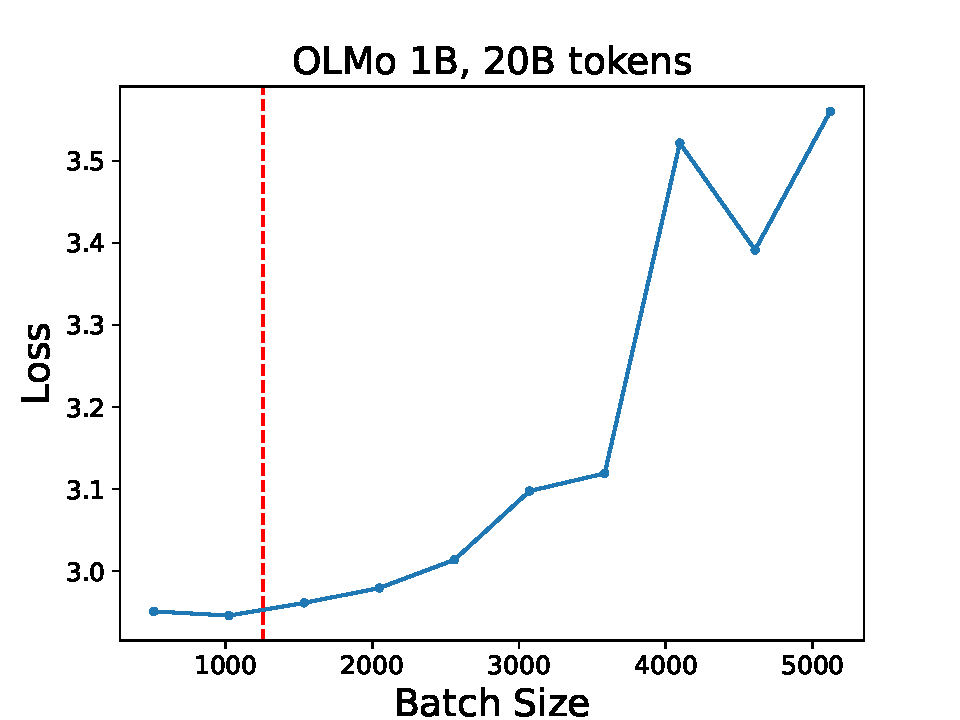
\includegraphics[width=0.32\linewidth]{figures/measure-cbs/peteish1-fixlr/from10000.pdf}
    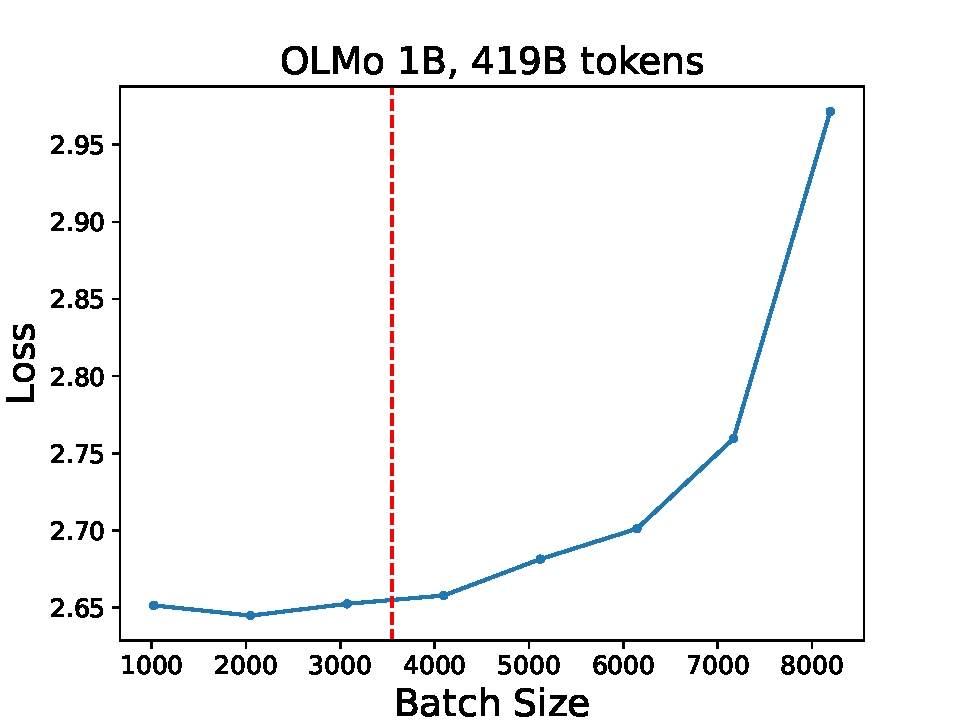
\includegraphics[width=0.32\linewidth]{figures/measure-cbs/peteish1-fixlr/from200000.pdf}
    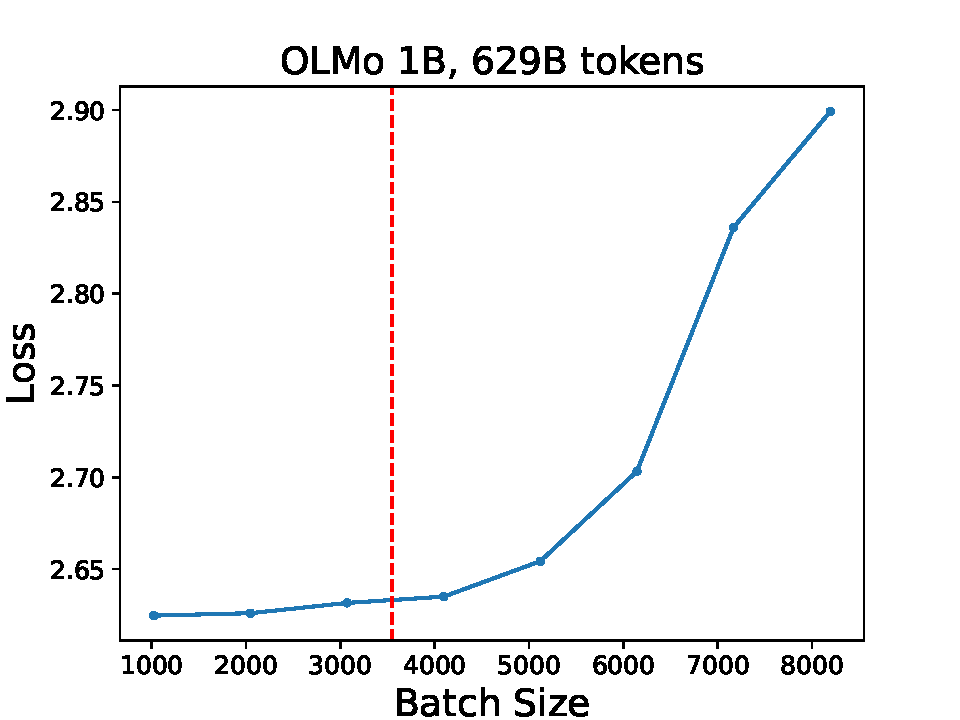
\includegraphics[width=0.32\linewidth]{figures/measure-cbs/peteish1-fixlr/from300000.pdf}
    \caption{Smoothed final loss after branched training at particular checkpoints, with $B^*$ shown as the dotted red line. Each point represents the loss achieved by a specific branched training run after 2B tokens. Our method detects the point at which loss starts to increase, heuristically tolerating noise within $\epsilon = 0.01$.
    These plots show how this plays out for three particular checkpoints; see \Cref{sec:cbs-measurement-details} for loss curves for all checkpoints.}
    \label{fig:loss-curves}
\end{figure}

Our method will empirically estimate the largest batch size $B^*$ at which the local optimization trajectory recovers roughly to its original loss after $\Delta$ steps.
In contrast to the strong assumptions needed to justify the gradient noise scale, the only (weak) assumption our method relies on is:

% \hanna{can we somehow justify that this assumption is reasonable? do we have some empirical curves to show this? } \WM{can't fully justify without launching full training runs. but, within the windows we're looking in, it does seem that once two losses converge they don't separate}
\begin{assumptionbox}{Local Recovery}
    If the loss achieved by batch size $B^*$ recovers to match the loss with batch size $B < B^*$ after training for $\Delta$ tokens, the loss trajectories will remain the same beyond $\Delta$ as well.
\end{assumptionbox}

\paragraph{Implementation Details.} Our method requires specifying two parameters: the window size $\Delta$ and the loss tolerance $\epsilon$.
We also apply smoothing to the loss to reduce noise.
In more detail:

\begin{compactenum}
    \item \textbf{Window Size.}
    Because the optimizer state must update when the batch size is changed, we expect an immediate spike in the loss after adjusting the batch size.
    The window size $\Delta$ represents the number of steps we are willing to wait for the loss to recover from this bump.
    The CBS measurements could, in principle, depend on $\Delta$, with larger values of $\Delta$ potentially producing larger CBS estimates.
    We set $\Delta$ to 2B tokens, which we take as a small, conversative window size relative to our overall pretraining budget of 600B tokens.

    \item \textbf{Loss Tolerance.} Viewing loss as a function of batch size multiplier $k$ (cf.\Cref{fig:loss-curves}), we need a way to determine whether the loss at $k^*$ has increased relative to all $k<k^*$. We operationalize this with a tolerance parameter $\epsilon$, which we set to 0.01 arbitrarily.
    In principle, tolerance could be set in a more principled way using a statistical test in future work.

    \item \textbf{Loss Smoothing.} Pretraining loss is noisy at the batch level, so, following standard practice, we apply exponentially moving average smoothing with parameter $\alpha$ set to 0.5.
\end{compactenum}

It is worth comparing our method to other work that empirically measures the CBS.
Our method of training for a fixed token budget $\Delta$ and measuring the change in loss can be understood as the dual view to measuring the number of steps required to achieve a target loss, which has been used in prior work \citep{zhang-2019-algorithmic,zhang2024cbs}.
Reformulating the measurement in this way has the nice property that the training budget can be fixed in advance.
Under the local recovery assumption, it also allows us to train for only $\Delta$ tokens, which means we do not have to launch full training runs for each batch size.
Finally, unlike \citet{zhang2024cbs}, we apply our method at various checkpoints throughout training, whereas they apply it only from initialization.
This means we can estimate the \emph{local CBS} at a specific point in training rather than just the \emph{global CBS}.

\subsection{Experimental Setup}

We aim to measure the CBS over the course of model training and the role of model size.
Because our method requires pretraining checkpoints and access to the pretraining data, we use the OLMo 1B and OLMo 7B models for our experiments \citep{olmo20252olmo2furious}, whose pretraining data is openly available \citep{soldaini2024dolma}.
For each model, we take a variety of checkpoints over the course of training, allowing us to assess how the CBS changes over the course of training; see \Cref{sec:cbs-measurement-details} for more details.
We also compute the noise scale across training checkpoints using the estimator proposed by \citet{mccandlish2018empirical} to assess whether it is a valid proxy for the CBS we measure.

We define the interval for the CBS at each checkpoint by choosing $B^*$ (as defined in \Cref{sec:our-method}) as a lower bound, and by picking the least $k > k^*$ as an upper bound. The plotted point represents the geometric mean of these interval endpoints.
We measure the CBS in documents, with a pretraining sequence length of 4096 tokens per document.

\subsection{Results: CBS Over Training and Across Model Sizes}

\begin{figure}
    \centering
    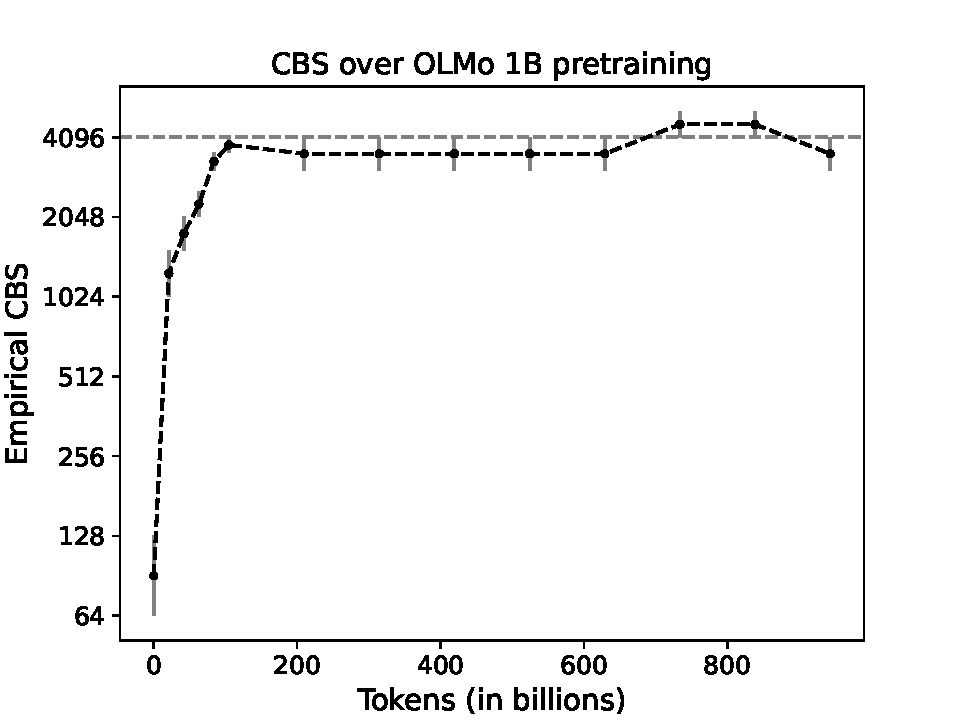
\includegraphics[width=0.48\linewidth]{figures/measure-cbs/peteish1-fixlr/main.pdf}
    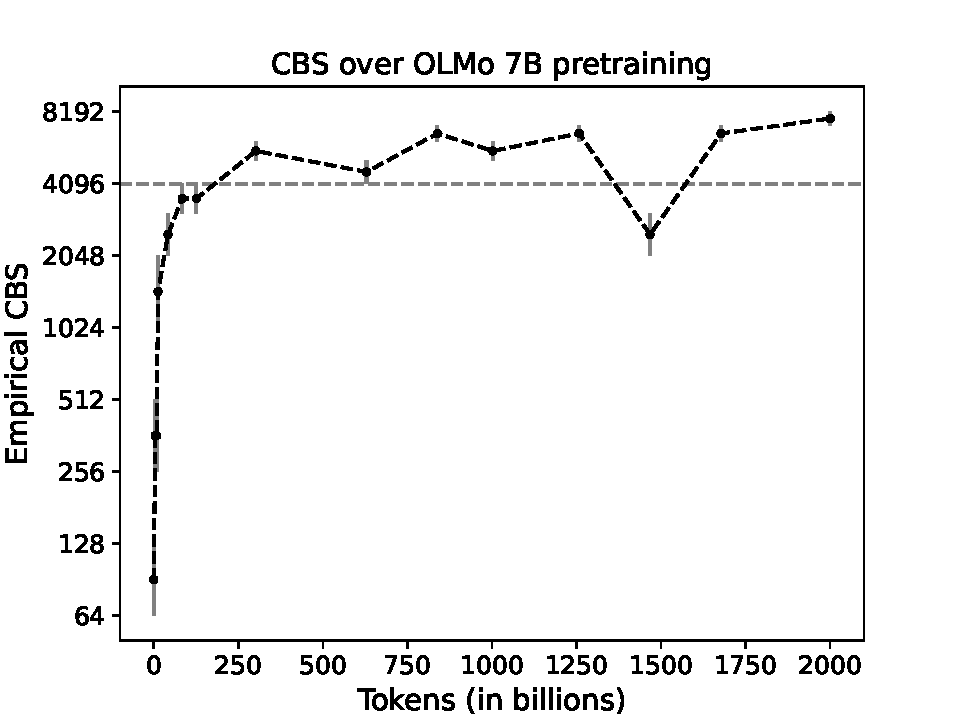
\includegraphics[width=0.48\linewidth]{figures/measure-cbs/peteish7/main.pdf}
    \caption{CBS over training for OLMo 1B and 7B, measured in documents (4096 tokens per document). The qualitative trend is similar across both model sizes. The CBS starts near 0, grows rapidly but diminishingly, and plateaus around 4096.}
    \label{fig:measure-cbs}
\end{figure}

\Cref{fig:measure-cbs} shows the CBS $B^*$ measured via \Cref{box:empirical-cbs} across training checkpoints for OLMo 1B and 7B.
The CBS increases over training in a similar way for both model sizes:
the CBS starts near 0, grows rapidly within the first 50k tokens, and then plateaus around 4096.

\paragraph{Impact of Model and Data Size.}
Prior work has suggested that the CBS is largely independent of model size, scaling primarily with data size \citep{zhang2024cbs,bergsma-2025-powerlines}.
This is largely consistent with our findings, as the CBS curves like qualitatively similar at the 1B and 7B scales.
In addition, the fact that the CBS grows over training suggests that the ``aggregate'' CBS should also increase as we train on more data since the average CBS over the course of training should increase.
We elaborate on this in \Cref{sec:scaling-laws}: while CBS growth over training predicts that aggregate CBS should increase with data size, it is unclear whether the CBS growth pattern we observe would predict the aggregate CBS $\propto \sqrt{D}$ scaling law found in prior work \citep{zhang2024cbs,bergsma-2025-powerlines}.

\paragraph{Comparison with Gradient Noise Scale.}
As discussed in \Cref{sec:noise-scale}, the gradient noise scale has been proposed as a proxy to measure the CBS \citep{mccandlish2018empirical}, though this connection relies on strong assumptions to justify.
We thus empirically compare our measurement of the CBS to the gradient noise scale.
\Cref{fig:noise-scale} shows that, for both OLMo 1B and 7B, the gradient noise scale underestimates the CBS by several orders of magnitude. Furthermore, especially for OLMo 7B, the qualitative trend does not match the CBS.
For OLMo 1B, the qualitative pattern is more similar.
However, since this similarity is not found for both models, we conclude that, in general, the noise scale cannot be used reliably as a proxy for the CBS.
% Since our method directly measures noise scale, our interpretation of this discrepancy is that the strong assumptions (\Cref{sec:noise-scale}) required to justify the noise scale proxy are problematic in practice, and thus that the noise scale is not a reliable way to estimate the CBS.

\begin{figure}
    \centering
    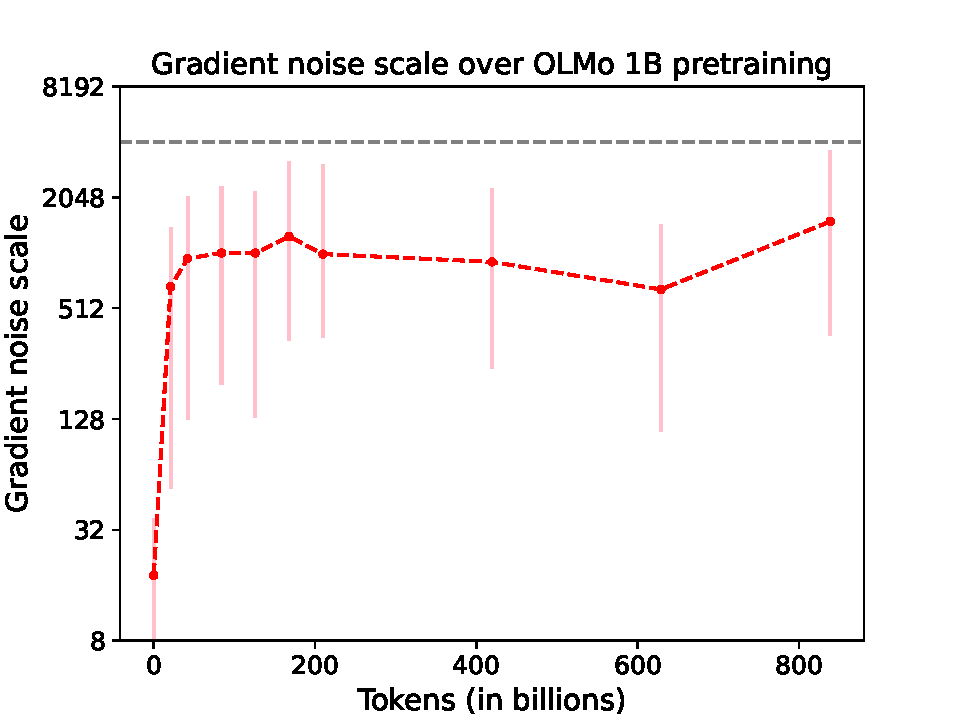
\includegraphics[width=0.48\linewidth]{figures/noise-scale/peteish1/noise-scale.pdf}
    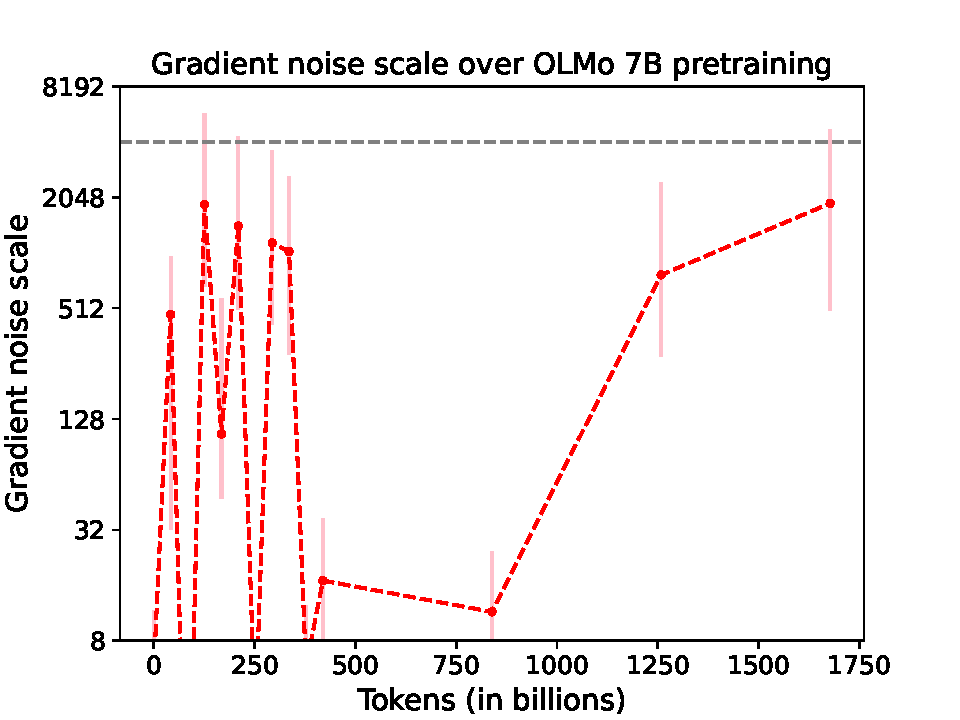
\includegraphics[width=0.48\linewidth]{figures/noise-scale/rel/noise-scale.pdf}
    \caption{Gradient noise scale for OLMo 1B and 7B computed via the estimator of \citet{mccandlish2018empirical} with 95\% confidence intervals; details in \Cref{app:noise-scale}.
    The gradient noise scale underestimates the CBS (cf.~\Cref{fig:measure-cbs}) and the qualitative trend does not clearly match, especially for OLMo 7B.}
    \label{fig:noise-scale}
\end{figure}

\paragraph{Motivating Batch Size Warmup.}
A central takeaway from these results is that the CBS starts near 0, grows rapidly, and then plateaus.
This suggests that \emph{batch size warmup}, where the batch size is dynamically increased over the beginning of a training run, is a natural way to increase the effective batch size for most of training while avoiding training with a batch size above the CBS.
In the next section, we will discuss our implementation and validation of this idea.

\section{Application: Batch Size Warmup for Larger Batch Training} \label{sec:batch-size-warmup}

A straightforward way to speed up training is to increase the batch size, and, as long as the new batch size is less than the CBS, we can be confident that the loss will be minimized about as effectively as before.
Thus, we can leverage knowledge of the CBS to speed up training.

Furthermore, our local knowledge of the CBS can be leveraged to do this more effectively than if we only had a global sense of the CBS.
If we simply increased a fixed batch size, this would mean that we are training with a batch size that is too large for a short period at the beginning of training, which could potentially destabilize training or degrade final performance. To get around this, we can use our measurement of the local CBS to ``warm up'' the batch size.
We will train at a smaller batch size for the beginning of training when the CBS is small, and then switch to a larger batch size once the CBS grows large enough.
More generally, we can aim to double the batch size whenever we determine the CBS has doubled.
This should allow us to benefit from training at a larger batch size for \emph{most} of training without training at a batch size that is too large at the beginning of training, which could degrade the final loss achieved by the training run.

\subsection{Methodology for Batch Size Warmup} \label{sec:batch-size-warmup-method}

Given an existing training run (at a small batch size), we aim to adapt it to achieve the the same final loss with fewer overall gradient steps (i.e., a larger batch size for most of training).
Assuming an original fixed batch size $B$ and base learning rate $\eta$, our method for training with \emph{batch size warmup} is as follows.
First, we use branched training CBS method (\Cref{sec:our-method}) to measure $B^*_t$, the CBS after training for $t$ tokens, using an existing checkpoint.
When training a new model, we set the batch size and and learning rate as follows:

\begin{methodbox}{Batch Size Warmup} \label{box:batch-size-warmup}
    \begin{enumerate}
        \item At $t = 0$, initialize the batch size to $B_0 = B$ and base learning rate to $\eta_0 = \eta$.
        \item After training for $t$ tokens, if we determine that the CBS exceeds the current batch size ($B^*_t > 2B_t$), we double the current batch size and update the base learning rate following the square-root scaling rule (cf.~\Cref{sec:our-method}):
        \begin{align*}
            B_{t+1} &= 2 B_t \\
            \eta_{t+1} &= \sqrt{2} \eta_t .
        \end{align*}
    \end{enumerate}
\end{methodbox}

This method will ensure that the batch size will increase over training \emph{safely}, i.e., never exceeding the CBS.
Since we found that the CBS increases quite rapidly at the beginning of training, this method will double the batch size twice early in training, reaching a maximum batch size of 4096 by 503B tokens.
This means that we will effectively train at a larger batch size for most of training compared to the original small-batch run.
But, crucially, we can be confident that the batch size will never increase our batch size above the CBS. Thus, we expect the final loss will be comparable to that of the original training across thet training trajectory.

\paragraph{Implementation Details.} The main implementation question is how to operationalize checking $B^*_t > 2B_t$ in order to double the batch size.
In practice, we do this heuristically based on the measurements in \Cref{fig:measure-cbs}: since we only double the batch size twice over training, this involves just picking two thresholds.
In addition, this process could be automated for future training runs using online measurements of the CBS paired with some kind of curve fitting or statistical test.

\paragraph{Design Choices.} As defined above, our method uses a square-root scaling rule, which is well-motivated for Adam \citep{malladi2022sdes}, but in principle a linear scaling rule could also be used.
As batch size warmup only modifies the base learning rate, it is compatible to overlay with existing learning rate schedules (in practice, the models we use follow a cosine schedule).
Finally, we choose to only increase the batch size at powers of two because it is not clear that having a more precise match to the CBS beyond the order-of-magnitude level would be particularly useful and because the OLMo codebase requires the number of GPUs $g$ divides the batch size.
\upd{Thus, doubling is convenient because it easily guarantees the new batch size remains a multiple of $g$.
However, in principle one could update more frequently, e.g., by setting updating the batch size the largest multiple of $g \leq B^*_t$.}
% \DG{OLMo doesn't enforce batch sizes that are powers of two. The problem is that the number of GPUs you have needs to divide the batch size evenly. If I want to write some code that can increase the batch size in a running job (and I don't want to make any assumptions about the
% existing batch size and number of GPUs I have), then doubling is the only thing I can do.}

\paragraph{Connection to Existing Methods.}
Our batch size warmup method is similar to preliminary experiments by \citet[Appendix D]{mccandlish2018empirical} using a dynamic batch size on the SVHN dataset. However, they use their noise scale method (\Cref{sec:noise-scale}) to set the batch size, which is potentially unreliable, and only consider small-scale classification.
In the context of image classification, prior work explored replacing learning rate decay with increasing the batch size \citep{smith-2018-decay}.
This is conceptually related to our batch size warmup approach in that it leverages scaling rules between batch size and learning rate to achieve larger batch training.
However, our method can apply on top of existing learning rate schedules, can generalize to Adam (vs.~SGD), and, most crucially, ensures that the batch size number exceeds the critical batch size.

\subsection{Experimental Setup}
%To showcase the impact of our batch size warmup method, our objective is to evaluate two claims.\hanna{rewrote these two sentences; check if that's accurate?}
%1) Training with our method should match the original small-batch-size run in terms of final loss.
%2) we expect our method to achieve better final loss than just training with a fixed batch size. 
%Therefore, we train a model with batch size warmup and compare it against these other approaches as controls, meaning we have the following experimental conditions:
We evaluate the viability of training with batch size warmup via the following training runs. For all models, we use the default OLMo 1B pretraining hyperparameters unless stated otherwise.

\begin{enumerate}
    \item \textbf{Batch Size Warmup:} We train OLMo 1B with our batch size warmup method as detailed in \Cref{sec:batch-size-warmup-method}.
    We initialize the batch size to 1024.
    Based on a manual reading of the CBS measurements in \Cref{sec:our-method}, we determine that the CBS reaches 2048 by 168B tokens and 4096 by 503B tokens.\footnote{\upd{These thresholds were determined from preliminary CBS measurements at an earlier stage of the project. Our measurements changed slightly after this point, but we deemed that it was not worth it to restart the expensive training runs because we do not think the results should be sensitive to a precise choice of threshold. Going forward, it could be useful to establish systematic methodology for choosing batch size warmup thresholds given the CBS measurements.}}
    Our method thus doubles the batch size at each of these points.
    \item \textbf{Small-Batch Control:} We train OLMo 1B with batch size $B = 1024$ and base learning rate $\eta = \sqrt{2} \cdot 0.0004$.\footnote{The default hyperparameters for OLMo 1B use a batch size of 512 and learning rate of 0.0004. Since we chose an initial base size of 1024 for our experiments, we adapted the learning rate appropriately via the square-root scaling rule \citep{malladi2022sdes}.}
    We expect that our batch size warmup method should be able to achieve similar final loss to the small-batch control with fewer gradient steps.
    \item \textbf{Large-Batch Control:} We train OLMo 1B with a fixed large batch size of $B = 4096$ and base learning rate $\eta = 2\sqrt{2} \cdot 0.0004$.
    Since its batch size will exceed the critical batch size for the initial part of training, we expect that the large-batch control will show degraded loss compared to our batch size warmup method.
\end{enumerate}

\begin{figure}
    \centering
    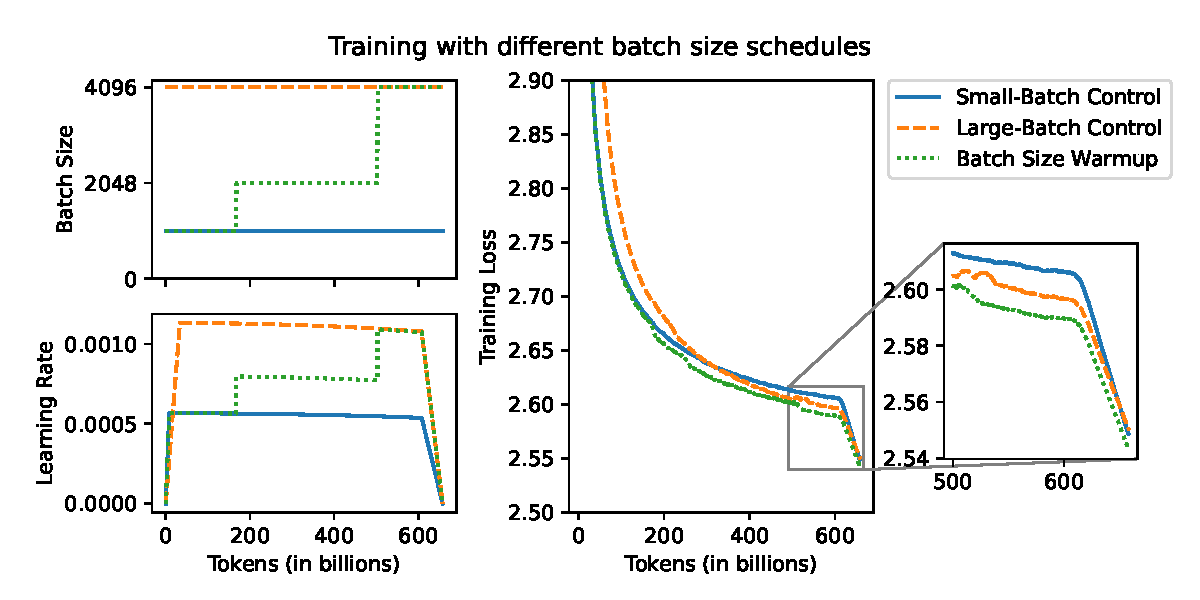
\includegraphics[width=0.98\linewidth]{figures/full-training/cbs-full.pdf}
    % \includegraphics[width=0.44\linewidth]{figures/full-training/cbs-lr.pdf}
    % \includegraphics[width=0.54\linewidth]{figures/full-training/cbs-loss.pdf}
    \caption{Batch size schedule (left, top), learning rate schedule (left, bottom) and training loss (right) for the pretraining of an OLMo model with different batch size schedules. Training loss is smoothed by taking the moving average over the past 10B tokens.}
    \label{fig:training-diff-methods}
\end{figure}

\begin{table}[!t]
    \centering
    \begin{tabular}{c|cc|c}
        \toprule
        Method & $\downarrow$ PT Loss & $\downarrow$ MT Loss & $\uparrow$ Grad.~Steps Saved \\
        \midrule
        Batch Size Warmup (Ours) & \textbf{2.5891} & \textbf{2.5433} & 43\% \\  % Steps: 1 - 89231/156921
        Small-Batch Control & 2.6057 & 2.5486 & 0\% \\ % Steps: 156921
        Large-Batch Control & 2.5962 & 2.5506 & \textbf{75\%} \\ % Steps: 1 - 39231/156921
        \bottomrule
    \end{tabular}
    \vspace{1em}
    \caption{Loss after pretraining (PT) and mid-training (MT) for each run, averaged over the past 10B tokens and the percentage of gradient steps saved vs.~the small-batch control (including annealing steps).
    Both before and after annealing, batch size warmup slightly outperforms both controls in loss.
    % Before annealing, batch size warmup outperforms both controls in loss, and after annealing, it is comparable in loss to the small-batch control.
    }
    \label{tab:loss-and-time}
\end{table}

\paragraph{Evaluations.} Language model training consists of two steps, pre-training and mid-training \citep{olmo20252olmo2furious}. We evaluate training loss as well as several measures of out-of-distribution loss at the end of the pre-training stage as well as after the mid-training stage.
\begin{compactitem}
    \item \textbf{Loss after Pretraining.} We evaluate the loss at the end of the pre-training stage for all models. 
    The original training run for OLMo 1B ran for 4T tokens, so we do not have the resources to replicate this full training run.
    Instead, we pre-train for 608B tokens using the original learning rate schedule for the longer run.
    % The simplest way to compare the losses of batch size warmup to our controls is at 600B tokens, i.e., partway through pretraining.
    \item \textbf{Loss after Mid-Training.}
    We report loss at the end of mid-training stage, which more closely reflects how these checkpoints are used in language model training. %which involves an additional step of In addition to comparing the loss at these partial checkpoints, we add an additional comparison using \emph{learning rate annealing}, 
    Specifically, starting from final pretraining checkpoint, we linearly anneal the remaining learning rate down to 0 for 50B tokens, keeping the batch size fixed at its final value (\Cref{fig:loss-curves}).
    Because mid-training is a part of the standard language modeling pipeline, we take the loss after mid-training to represent the loss that would be achieved by these training runs in a practical context.
    Furthermore, \citet{olmo20252olmo2furious} suggest that this kind of learning rate annealing can induce significant gains in loss for partial pretraining runs.
    We thus also take the loss after mid-training loss as a proxy for how these runs would compare if we were to fully train them for the full learning rate schedule.

    \item \textbf{Out-of-Distribution Losses.}
    To measure performance beyond the training loss, we also track three kinds of out-of-distribution losses.
    The first two are straightforward cross-entropy losses on common pretraining datasets, C4~\citep{C4} and The Pile~\citep{Pile}.
    The third out-of-distribution loss follows the method from \cite{Bhagia2024EstablishingTS}, which argues for computing the loss (in bits-per-byte; BPB) on the correct answers of multiple popular question-answering datasets such as ARC-Easy, ARC-Challenge, MMLU, etc. For the full list of datasets used, see Appendix \ref{app:bpb}.
\end{compactitem}

\subsection{Batch Size Warmup Results}

\begin{table}[!t]
    \centering
    \begin{tabular}{c|cc|cc|cc}
        \toprule
        Method & \multicolumn{2}{c}{$\downarrow$ Task BPB} & \multicolumn{2}{|c|}{$\downarrow$ C4} & \multicolumn{2}{|c}{$\downarrow$ Pile} \\
        & PT & MT & PT & MT & PT & MT \\
        \midrule
        Batch Size Warmup (Ours) & 1.0316 & 1.0076 & \textbf{2.8049} & \textbf{2.7597} & \textbf{2.1916} & 2.1521 \\
        Small-Batch Control & \textbf{1.0112} & \textbf{0.9999} & 2.8196 & 2.7622 & 2.2073 & \textbf{2.1471} \\
        Large-Batch Control & 1.0571 & 1.01927 & 2.8107 & 2.7658 & 2.1996 & 2.1586 \\
        \bottomrule
    \end{tabular}
    \vspace{1em}
    \caption{According to the method from \cite{Bhagia2024EstablishingTS}, we evaluate downstream performance via BPB on downstream tasks, as well as cross-entropy loss on two held-out sets, C4 and the Pile, both after pretraining and after mid-training.
    Batch-size warmup generally performs comparably or better compared to the small-batch control, suggesting it does not degrade downstream performance.
    }
    \label{tab:downstream}
\end{table}

We compare batch size warmup to the small and large-batch controls at two points: first, after the pretraining stage and, second, after the mid-training stage that anneals the remaining learning rate down to 0.
After pretraining, batch size warmup reaches lower loss than both controls, as shown in \Cref{fig:measure-cbs} and \Cref{tab:loss-and-time}, outperforming the small-batch control in loss by a margin of 0.0166.
After mid-training, batch size warmup still slightly outperforms the small-batch control in loss, this time by a smaller margin of 0.0053.
The large-batch control now achieves the worst overall loss.
% 
Overall, batch size warmup slightly exceeds the small-batch control in loss while using 43\% fewer gradient steps.
In contrast, the large-batch control uses 75\% fewer gradient steps, but its final loss degrades compared to the small-batch control.
Thus, we find batch size warmup is a reliable method to train with fewer gradient steps without degrading final loss.
% These results suggest that batch size warmup is a promising method for large-batch training that not only matches small-batch performance, but, possibly, improves it.

% Training with a larger batch size outperforms the small-batch control.
% \hanna{then second paragraph say: surprisingly, we see that small is worse than large before annealing, and the rest of the points. }

Beyond the final loss, we also evaluate whether batch size warmup leads to similar downstream performance as small-batch training using our downstream-task BPB evaluation as well as validation loss on C4 and the Pile.
% Precisely evaluating the impact of pretraining choices on downstream performance is an unsolved problem, but, following the advice of \citet{Bhagia2024EstablishingTS}, we evaluate downstream performance using bits per byte (BPB) on downstream task data as well as validation loss on C4 \citep{raffel-2020-exploring} and the Pile.
As shown in \Cref{tab:downstream}, we find that BPB on validation sets is broadly competitive with the small-batch control, performing best on three out of four conditions considered.
With the caveat that precisely measuring the downstream impact of pretraining decisions is difficult, this suggests that, just as batch-size warmup does not degrade final loss, it should not degrade downstream measures of performance either.

\section{Conclusion}

In this work, we introduced a simple empirical method for estimating the CBS throughout language model pretraining runs, which can be used to increase batch size (and thus effective token throughput) for large scale training runs without sacrificing performance.
As we discussed, the existing noise scale method \citep{mccandlish2018empirical} for estimating the CBS requires strong assumptions to justify, which our approach avoids.
We used our method to study the evolution of the CBS during training for the OLMo models, finding that CBS increases monotonically but diminishing over the course of training, and that CBS does not seem to depend on model size, in line with prior work \citep{zhang2024cbs}.
Guided by these findings, we showed that our measurements could be used to pick a \textbf{batch size warmup} schedule that enables larger batch training without harming final training loss.
We take these results to demonstrate the validity and utility of our CBS measurement approach, and believe our framework could be useful for increasing the efficiency of future large-scale pretraining efforts.

\upd{There are several details and extensions of our method that would be interesting to explore going forward.
First, it would be interesting to carry out a more systematic analysis of the impact of the hyperparameter $\Delta$ on CBS measurements: how sensitive is the method to $\Delta$ and do different values for $\Delta$ potentially bias the measurement?
It would also be interesting to further investigate the conditions under which noise scale might be a meaningful CBS proxy and used for batch size warmup.
When applying our CBS measurements to picking a batch size warmup schedule, we manually picked doubling threshold based on the CBS.
Going forward, it would be useful to establish a systematic way to set threshold for increasing the batch size given CBS measurements.
There are also other potential methodological improvements, such as removing the arbitrary power of 2 constraint and estimating the CBS in an online fashion.
Overall, these improvements would allow batch size warmup to be applied more robustly and easily across different pretraining setups.}

\section*{Acknowledgments}

We thank Joel Hestness, Sadhika Malladi, and Ananya Harsh Jha for discussions.

\bibliographystyle{abbrvnat}
\bibliography{references}

\clearpage
\appendix
\section{CBS Measurement Details} \label{sec:cbs-measurement-details}

Our empirical method for measuring the CBS \Cref{sec:our-method} is, in principle, sensitive to the choice of checkpoints and batch size multipliers.
We therefore document the checkpoints and multipliers we used here.

\paragraph{OLMo 1B.}
When measuring the OLMo 1B CBS with branching, we set the base batch size to 1024 and the base learning rate to $0.0004 \cdot \sqrt{2}$, reflecting the default batch size of 512 and learning rate of 0.0004 in the OLMo codebase under a square-root scaling rule \citep{malladi2022sdes}.
We then chose the following checkpoints and multipliers $k$:
\begin{enumerate}
    \item Step 0: $k$ ranging over 0.0625, 0.125, 0.25.
    \item Steps 10K, 20K, $\ldots$, 50K: $k$ ranging over 0.5, 1, $\ldots$, 5.
    \item Steps 100K, 150K, $\dots$, 450K: $k$ ranging over 1, 2, $\ldots$, 8.
\end{enumerate}
\Cref{fig:all-losses-1b} shows loss vs.~batch size plots for all checkpoints of OLMo 1B.

\paragraph{OLMo 7B.} We set the base batch size to 1024 and the base learning rate to $0.0003$, as specified in the OLMo codebase.
We then chose the following checkpoints and multipliers $k$:
\begin{enumerate}
    \item Step 0: $k$ ranging over 0.0625, 0.125, 0.25.
    \item Steps 1K, 2K, 3K: $k$ ranging over 0.25, 0.5, 1, 2, 3, 4.
    \item Steps 10K, 20K, 30K: $k$ ranging over 1, 2, 3, 4, 5.
    \item Steps 72K, 150K, 200K, 239K, 300K, 350K, 400K, 477K: $k$ ranging over 1, 2, 3, 4, 5, 6, 7, 8.
\end{enumerate}
\Cref{fig:all-losses-7b} shows loss vs.~batch size plots for all checkpoints of OLMo 7B.
These checkpoints were chosen manually as we developed this project.
Over the course of our experimentation, we launched many additional runs beyond the ones discussed above.
Since the choice of $k$ can influence the conclusions of our method, we filtered down the included runs to make the choice of $k$ systematic.

1B runs were launched on a single node of H100 GPUs, and 7B runs were launched on 8 nodes.

\begin{figure}
    \centering
    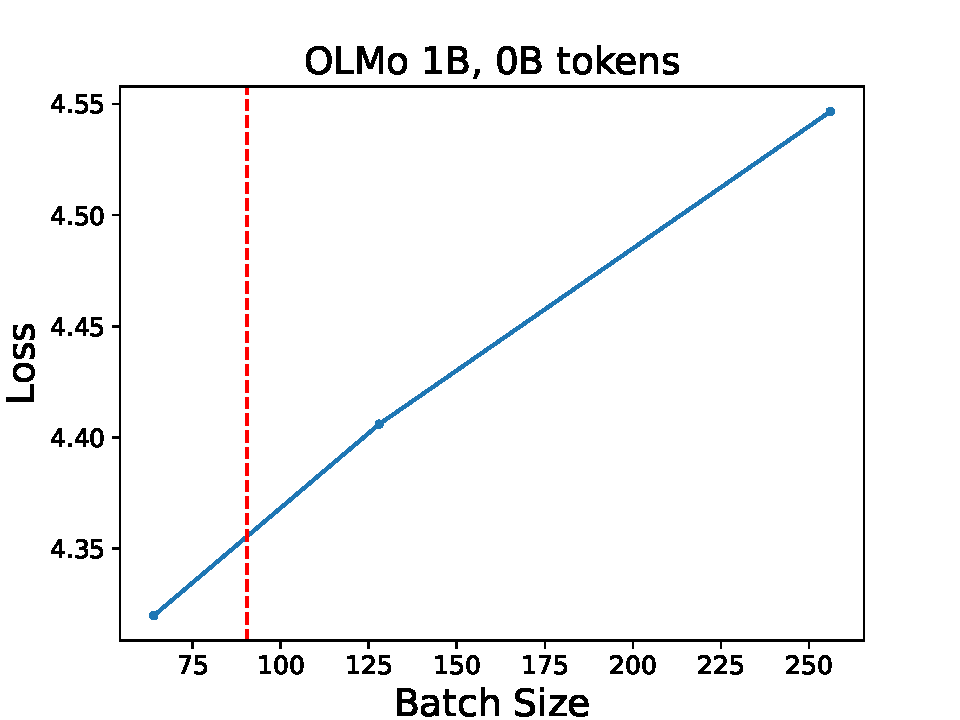
\includegraphics[width=0.32\linewidth]{figures/measure-cbs/peteish1-fixlr/from0.pdf}
    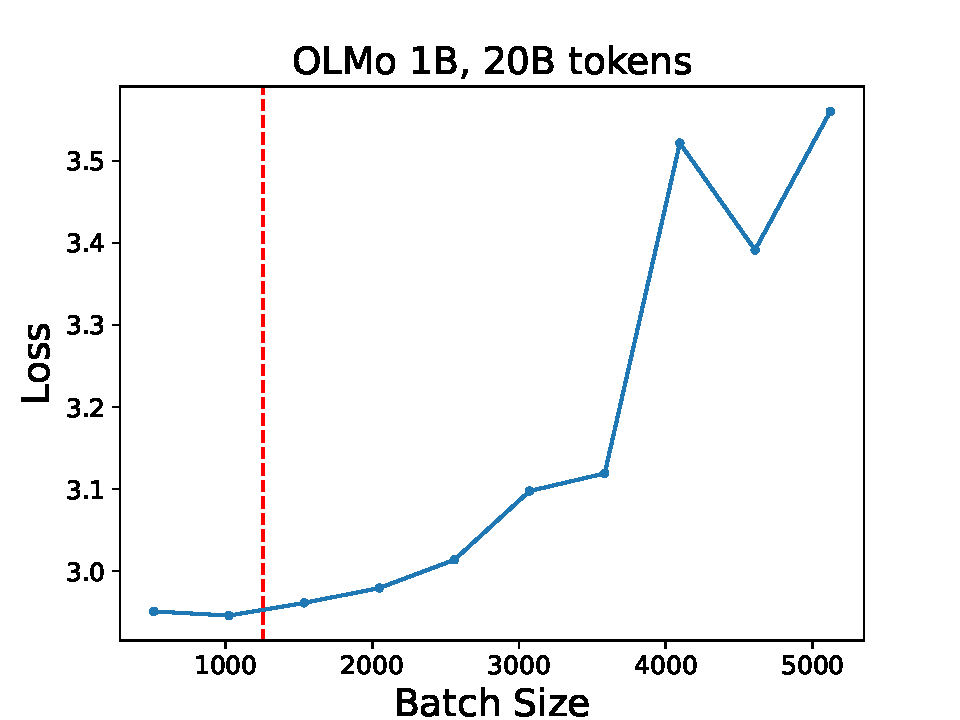
\includegraphics[width=0.32\linewidth]{figures/measure-cbs/peteish1-fixlr/from10000.pdf}
    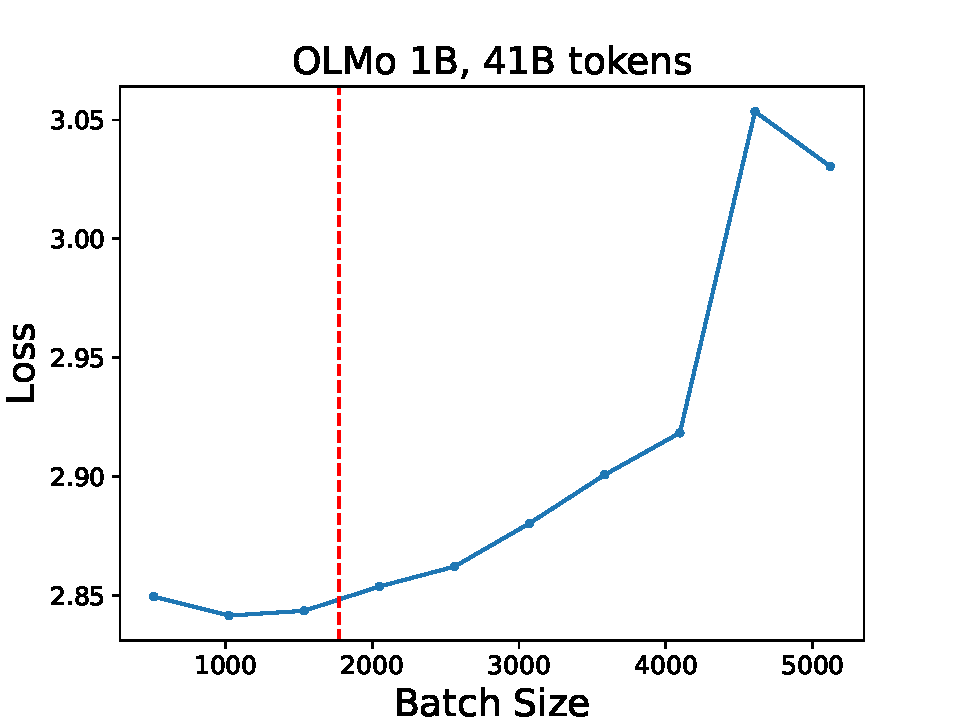
\includegraphics[width=0.32\linewidth]{figures/measure-cbs/peteish1-fixlr/from20000.pdf}
    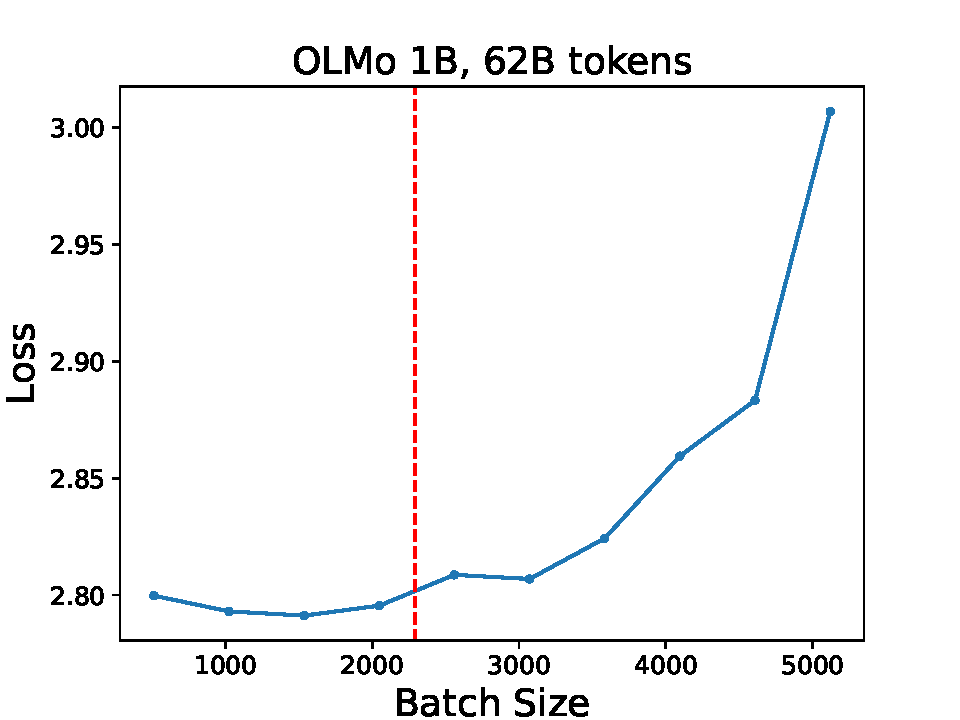
\includegraphics[width=0.32\linewidth]{figures/measure-cbs/peteish1-fixlr/from30000.pdf}
    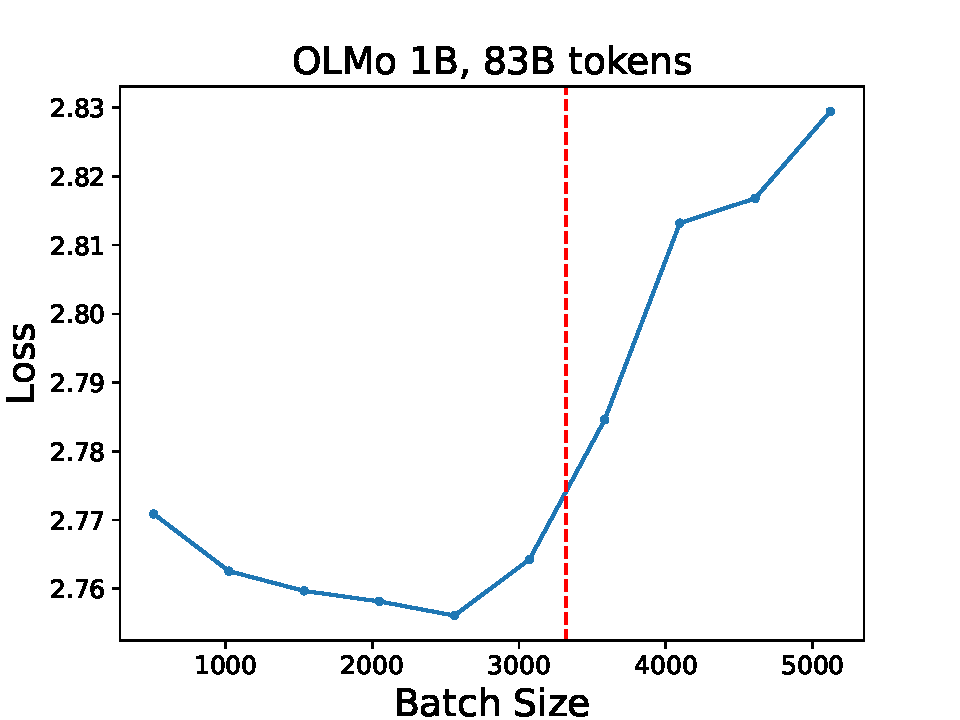
\includegraphics[width=0.32\linewidth]{figures/measure-cbs/peteish1-fixlr/from40000.pdf}
    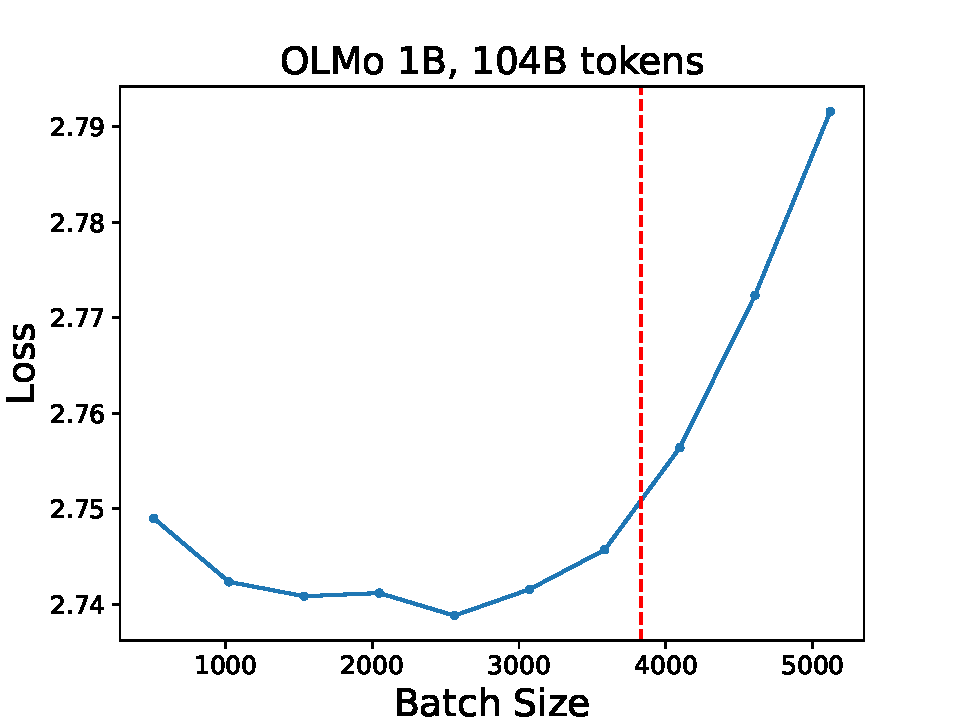
\includegraphics[width=0.32\linewidth]{figures/measure-cbs/peteish1-fixlr/from50000.pdf}
    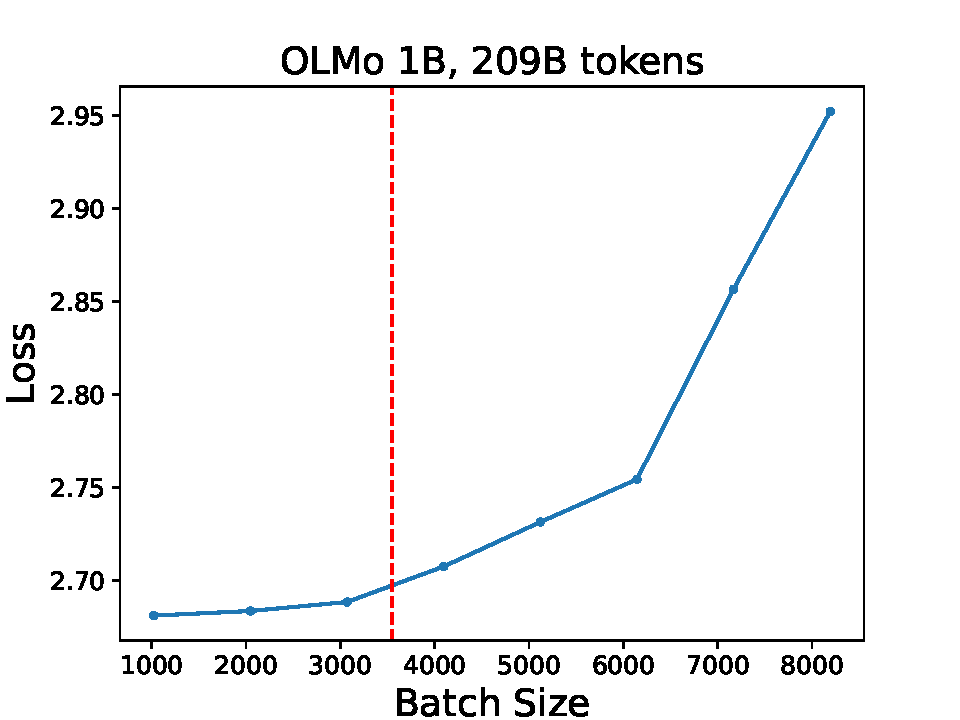
\includegraphics[width=0.32\linewidth]{figures/measure-cbs/peteish1-fixlr/from100000.pdf}
    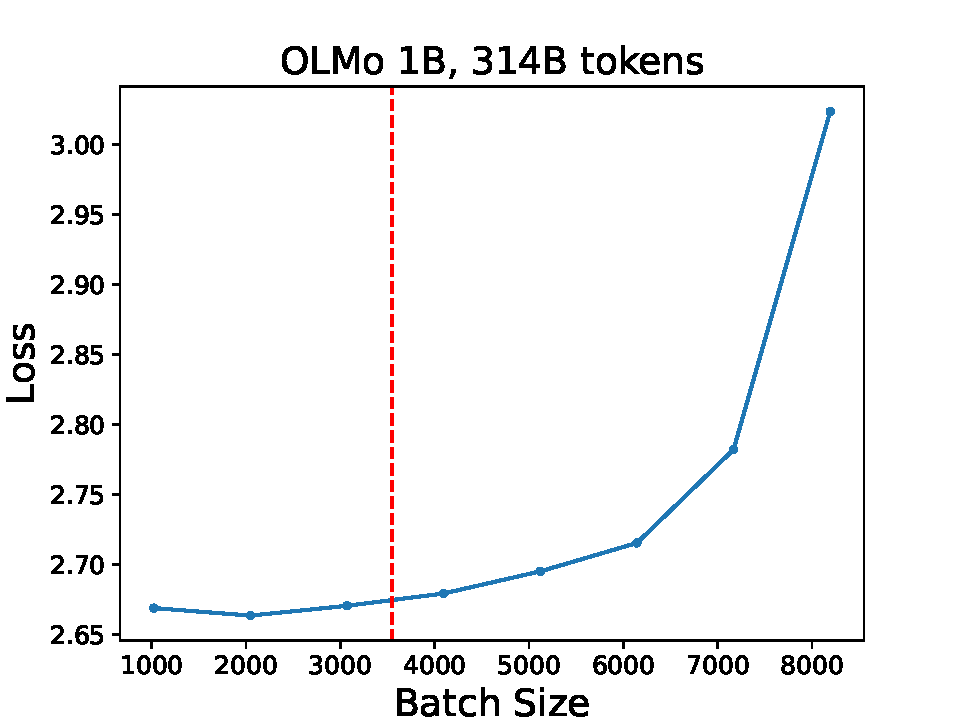
\includegraphics[width=0.32\linewidth]{figures/measure-cbs/peteish1-fixlr/from150000.pdf}
    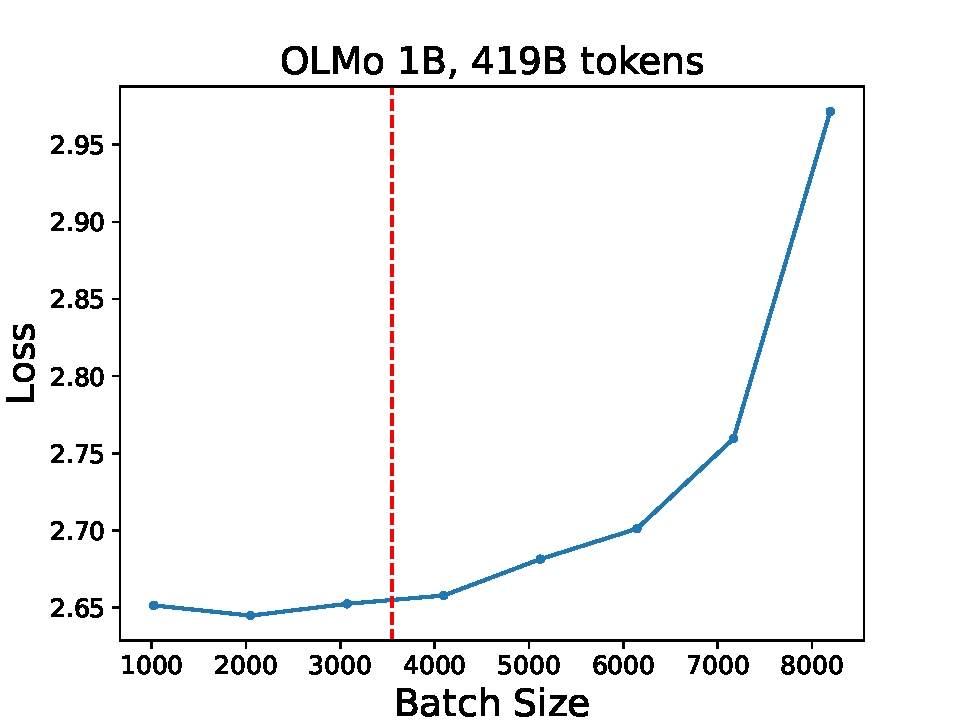
\includegraphics[width=0.32\linewidth]{figures/measure-cbs/peteish1-fixlr/from200000.pdf}
    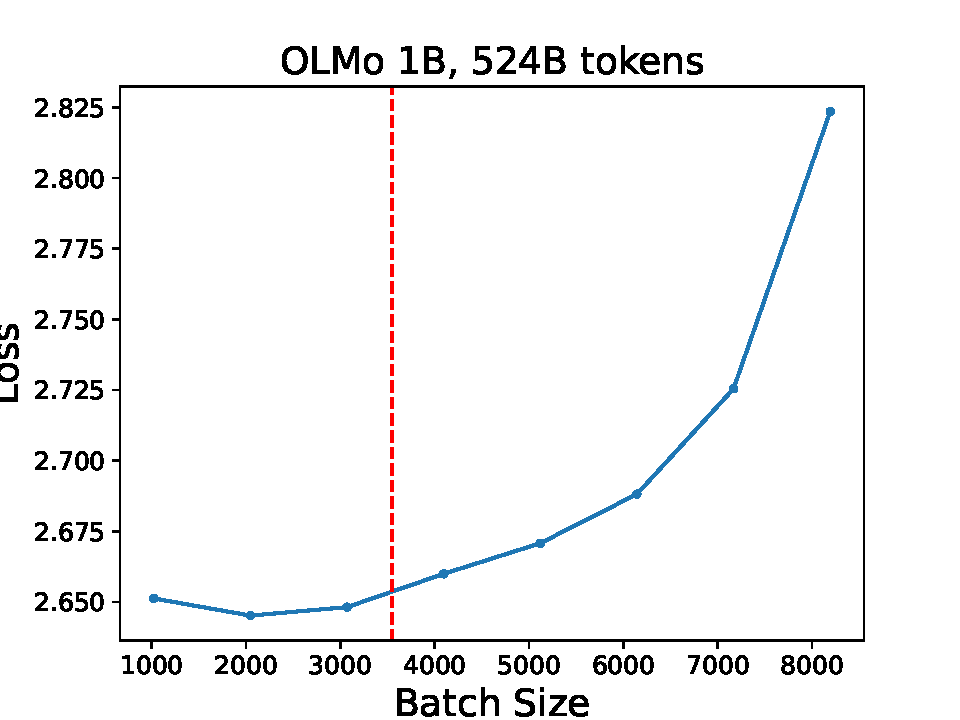
\includegraphics[width=0.32\linewidth]{figures/measure-cbs/peteish1-fixlr/from250000.pdf}
    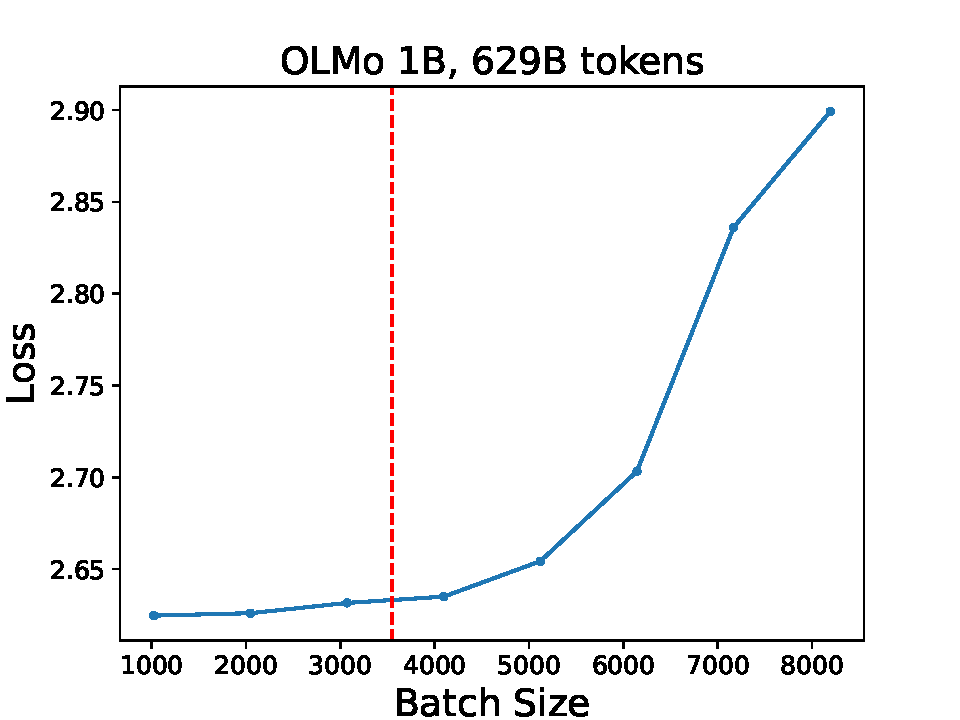
\includegraphics[width=0.32\linewidth]{figures/measure-cbs/peteish1-fixlr/from300000.pdf}
    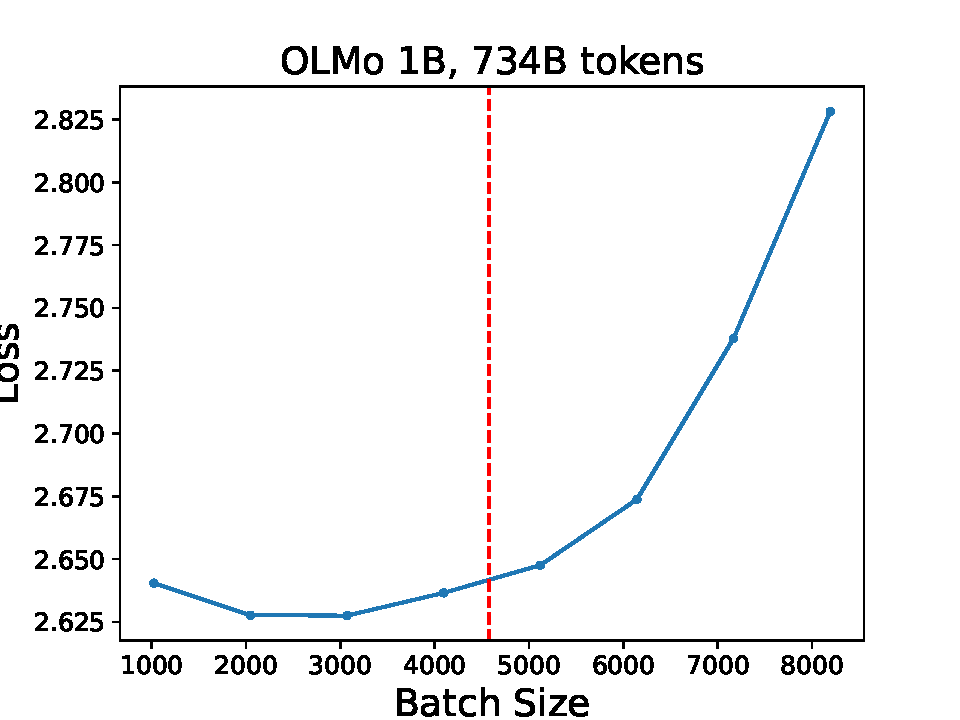
\includegraphics[width=0.32\linewidth]{figures/measure-cbs/peteish1-fixlr/from350000.pdf}
    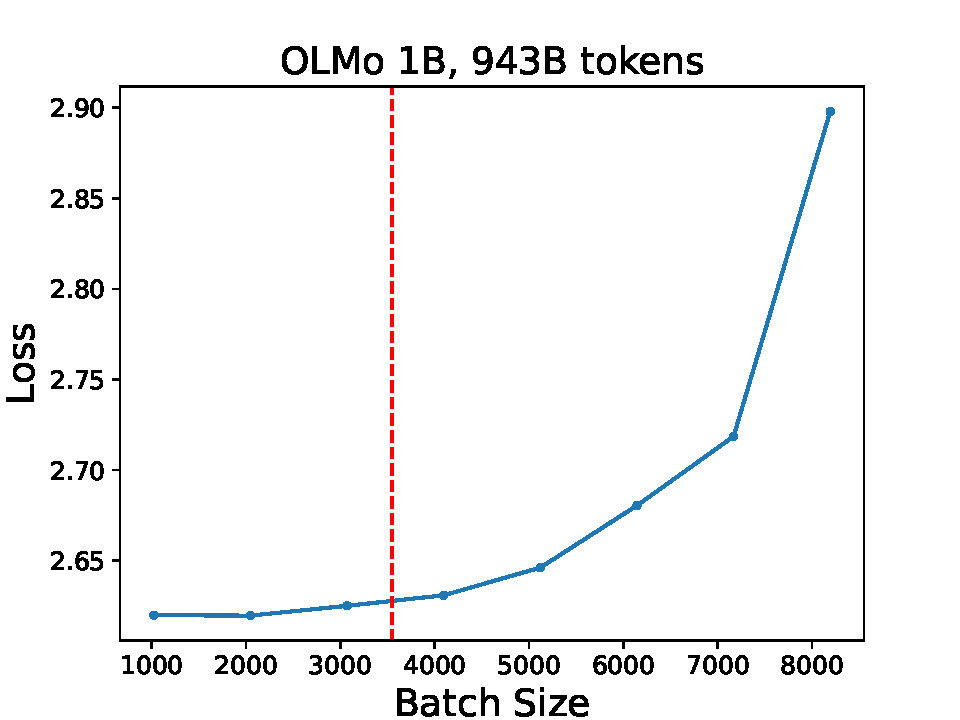
\includegraphics[width=0.32\linewidth]{figures/measure-cbs/peteish1-fixlr/from450000.pdf}
    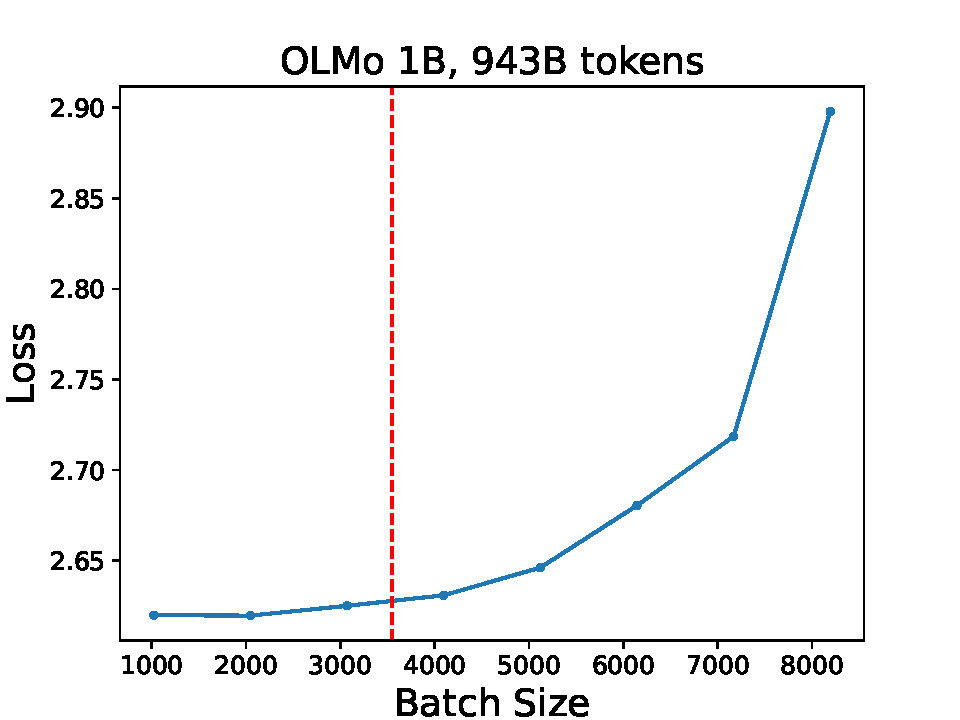
\includegraphics[width=0.32\linewidth]{figures/measure-cbs/peteish1-fixlr/from450000.pdf}
    \caption{All loss vs. batch size plots for OLMo 1B. Overall, the red line moves to the right over time, showing that the CBS increases.}
    \label{fig:all-losses-1b}
\end{figure}

\begin{figure}
    \centering
    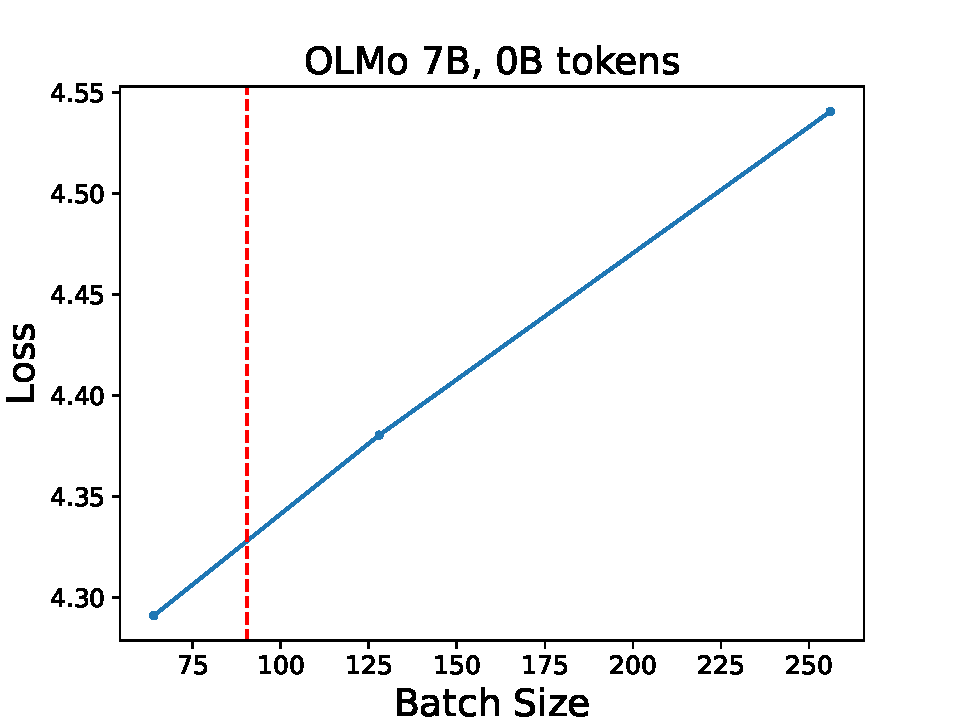
\includegraphics[width=0.32\linewidth]{figures/measure-cbs/peteish7/from0.pdf}
    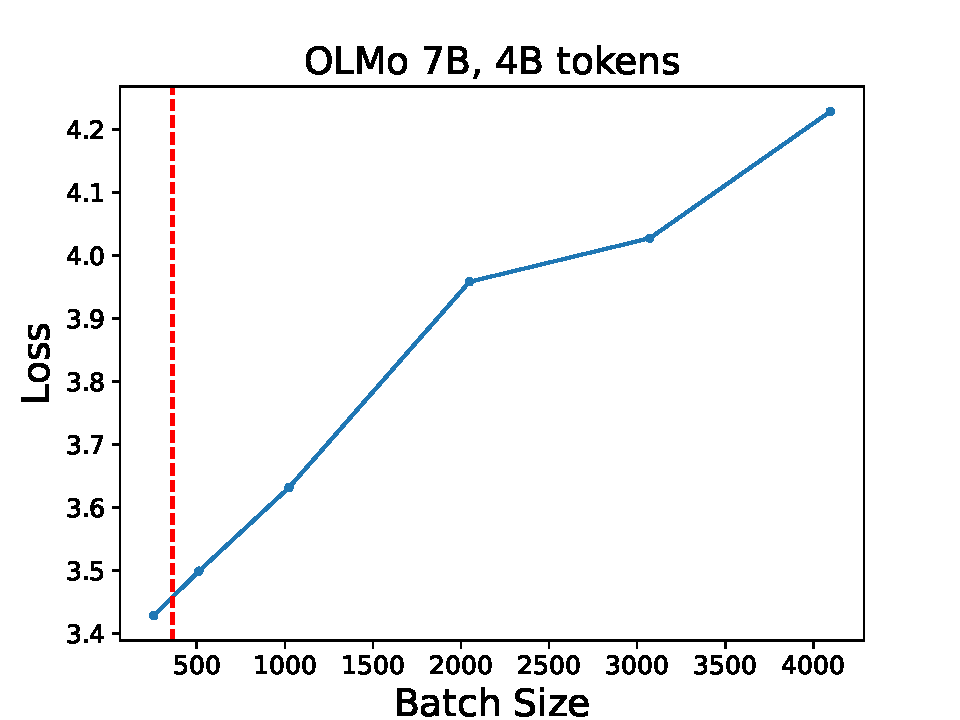
\includegraphics[width=0.32\linewidth]{figures/measure-cbs/peteish7/from1000.pdf}
    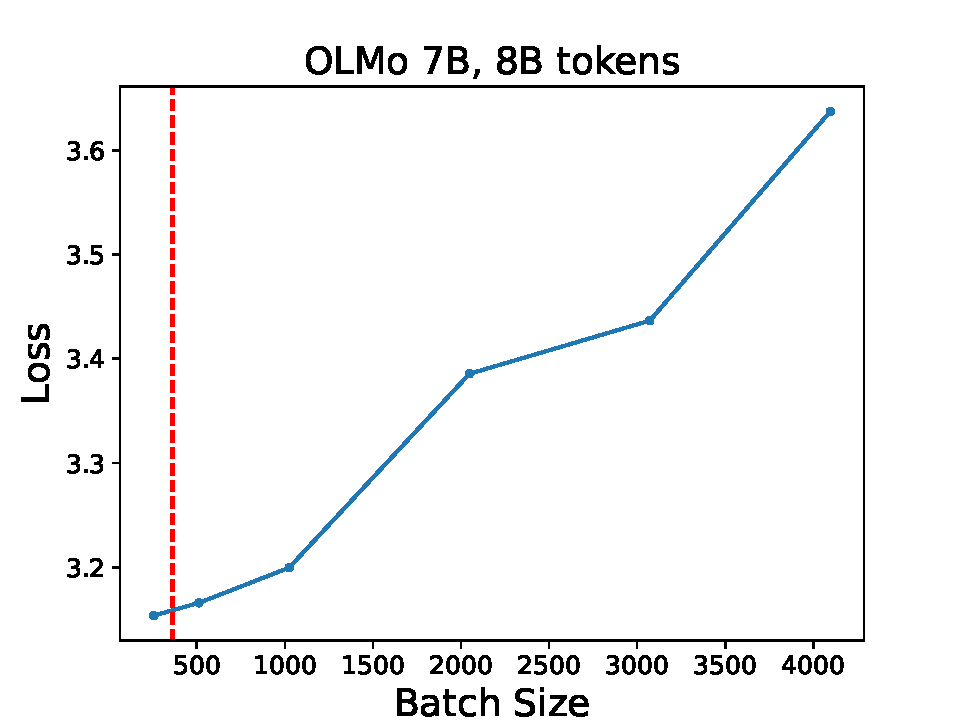
\includegraphics[width=0.32\linewidth]{figures/measure-cbs/peteish7/from2000.pdf}
    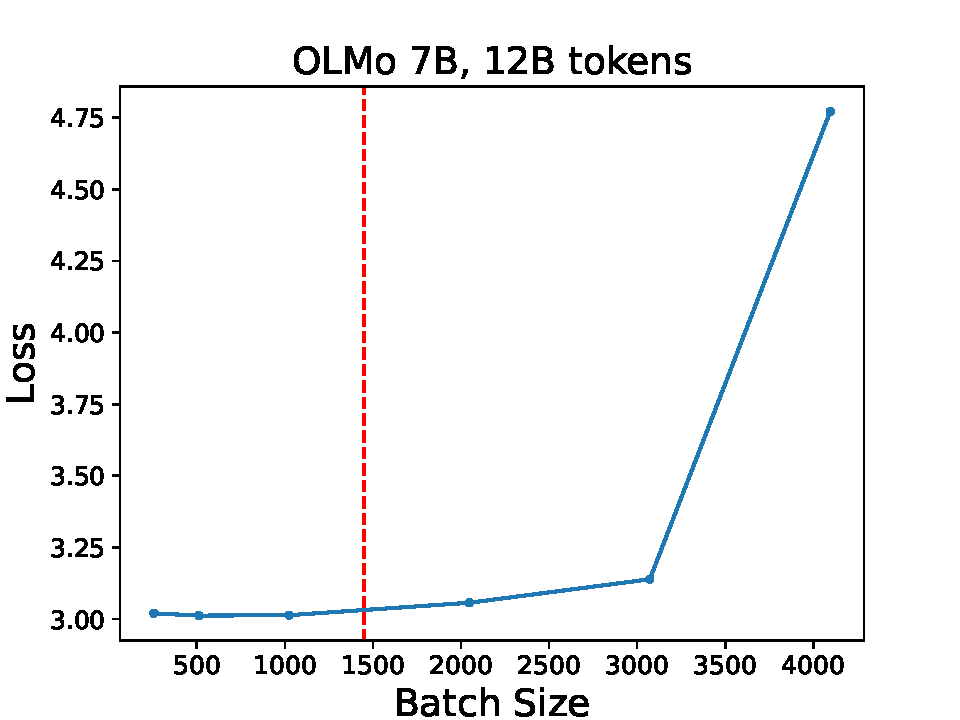
\includegraphics[width=0.32\linewidth]{figures/measure-cbs/peteish7/from3000.pdf}
    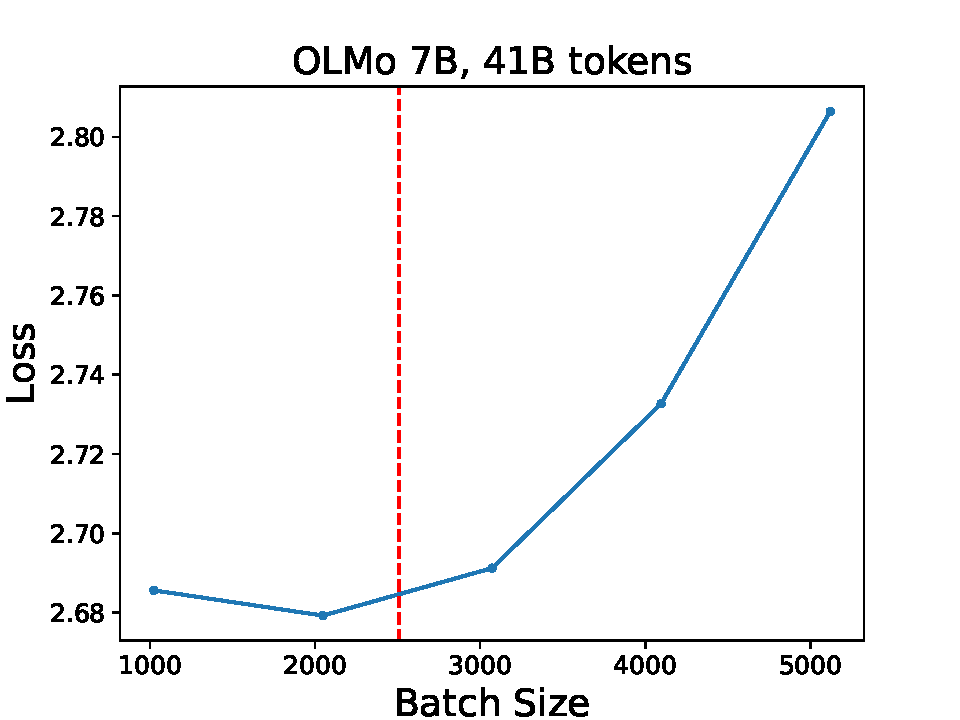
\includegraphics[width=0.32\linewidth]{figures/measure-cbs/peteish7/from10000.pdf}
    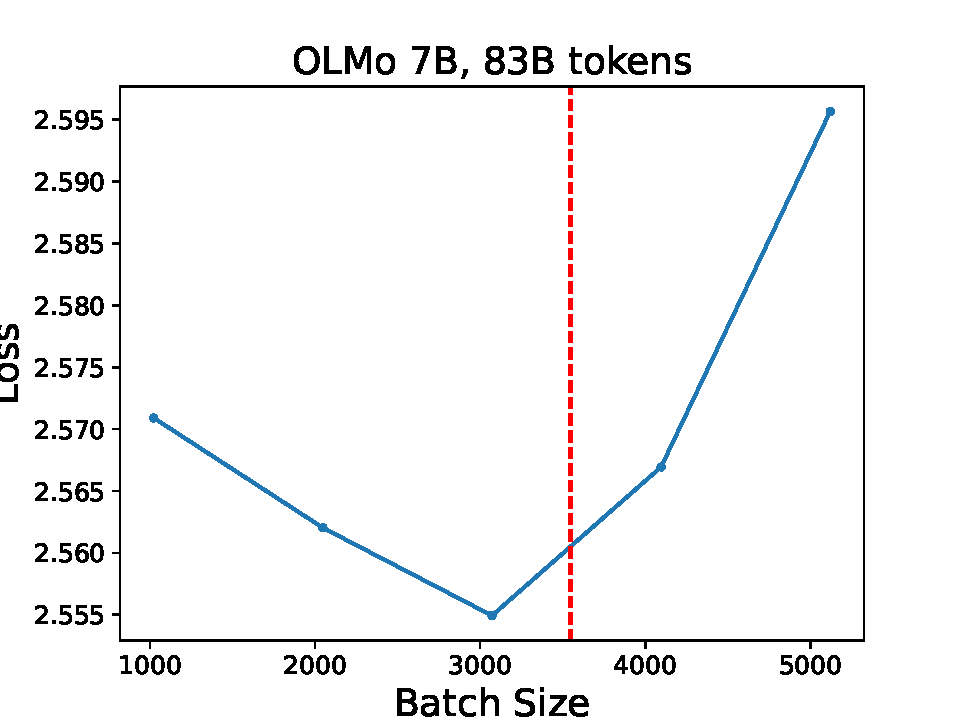
\includegraphics[width=0.32\linewidth]{figures/measure-cbs/peteish7/from20000.pdf}
    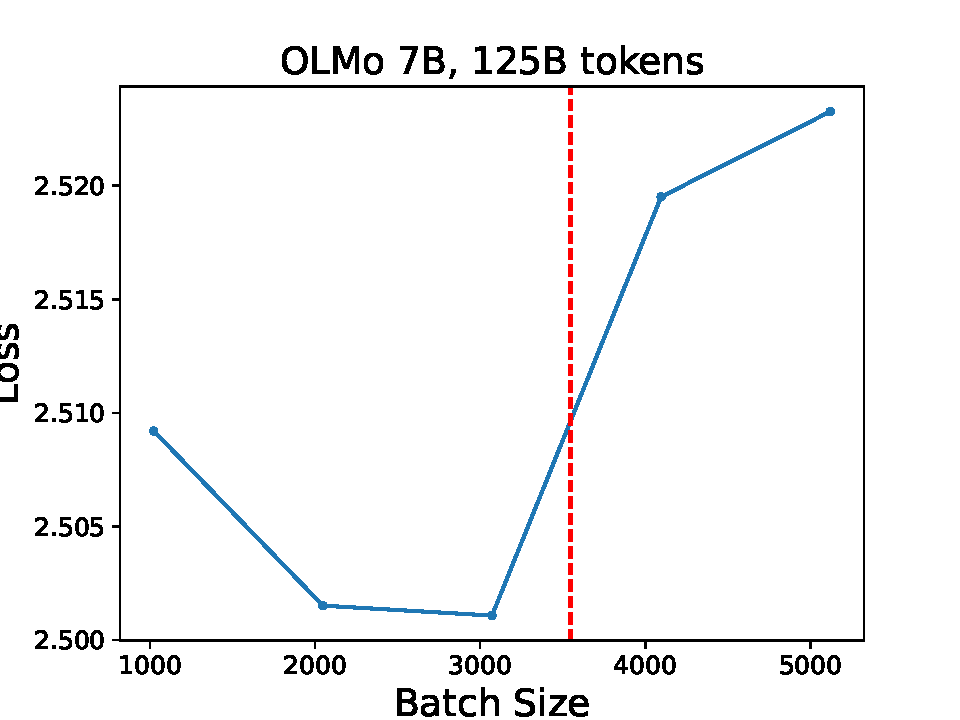
\includegraphics[width=0.32\linewidth]{figures/measure-cbs/peteish7/from30000.pdf}
    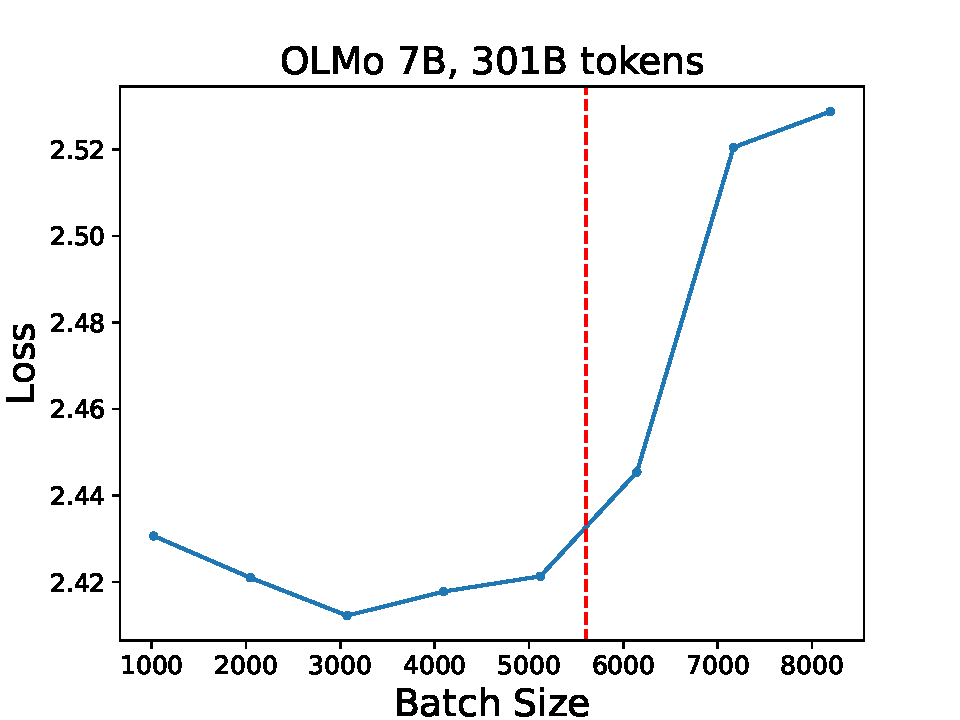
\includegraphics[width=0.32\linewidth]{figures/measure-cbs/peteish7/from72000.pdf}
    % \includegraphics[width=0.32\linewidth]{figures/measure-cbs/peteish7/from100000.pdf}
    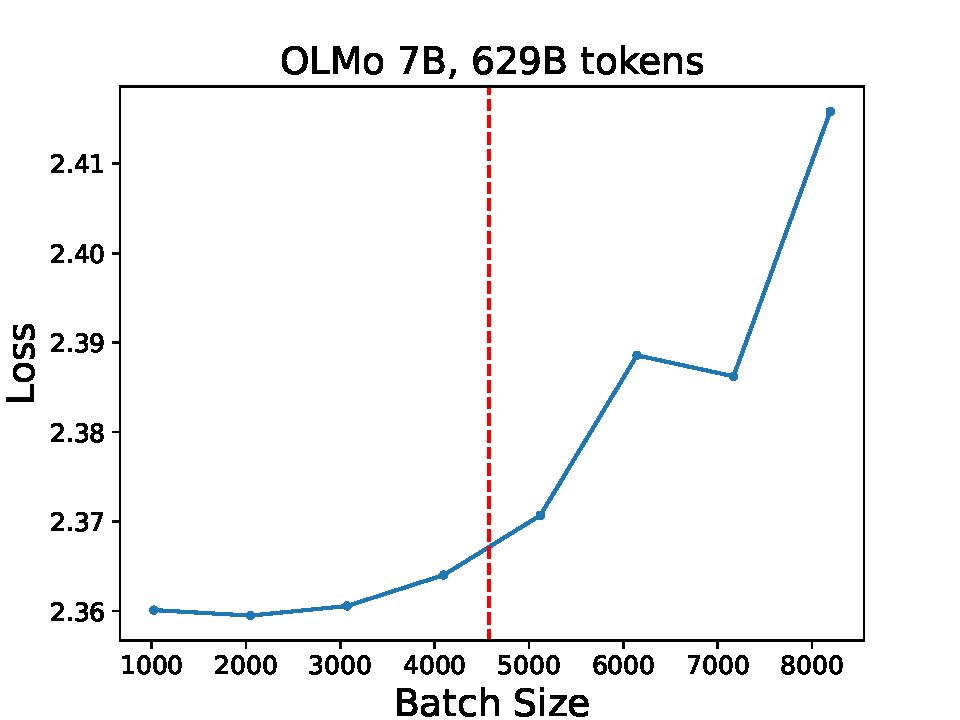
\includegraphics[width=0.32\linewidth]{figures/measure-cbs/peteish7/from150000.pdf}
    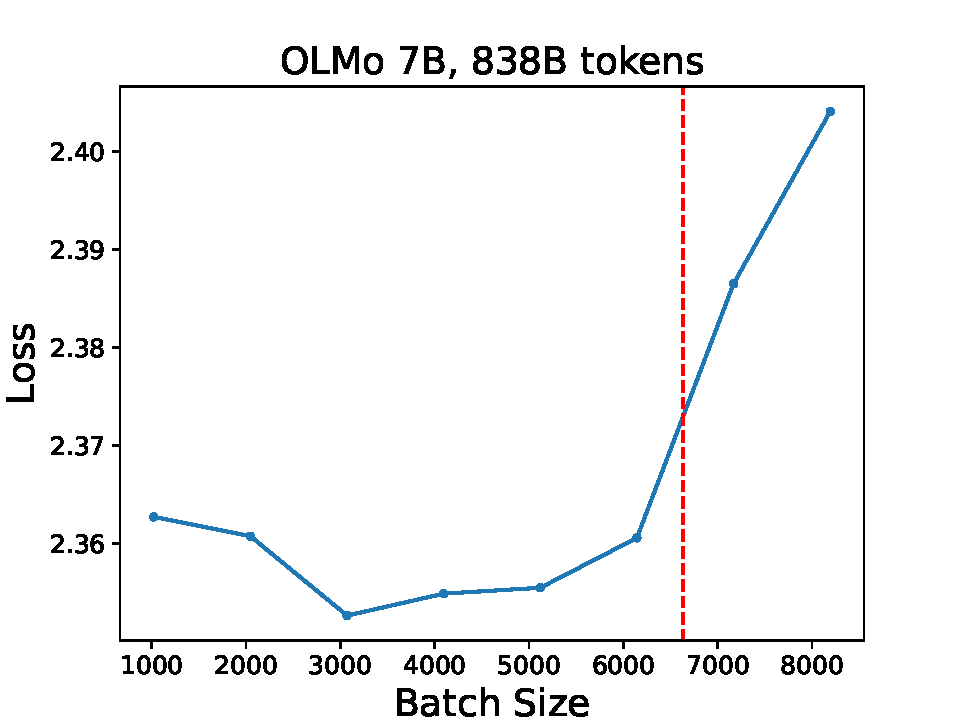
\includegraphics[width=0.32\linewidth]{figures/measure-cbs/peteish7/from200000.pdf}
    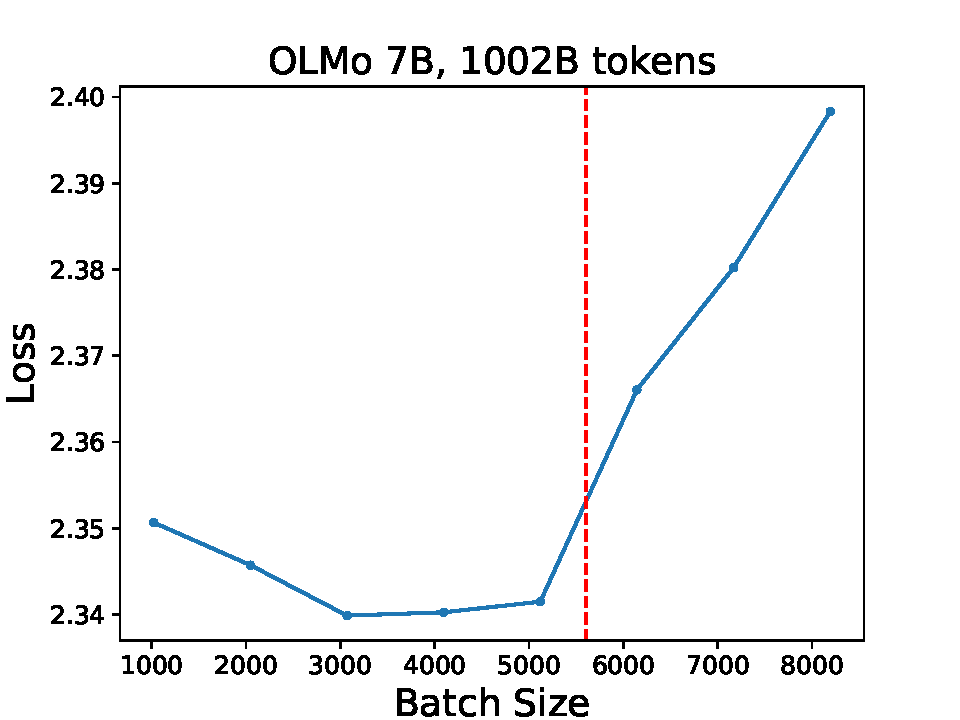
\includegraphics[width=0.32\linewidth]{figures/measure-cbs/peteish7/from239000.pdf}
    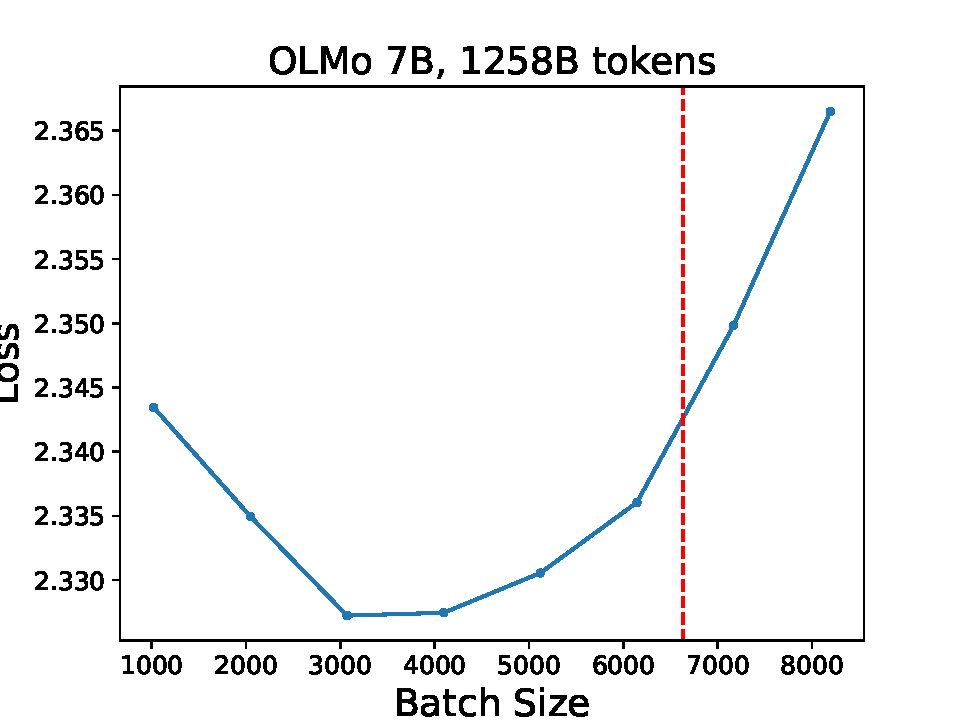
\includegraphics[width=0.32\linewidth]{figures/measure-cbs/peteish7/from300000.pdf}
    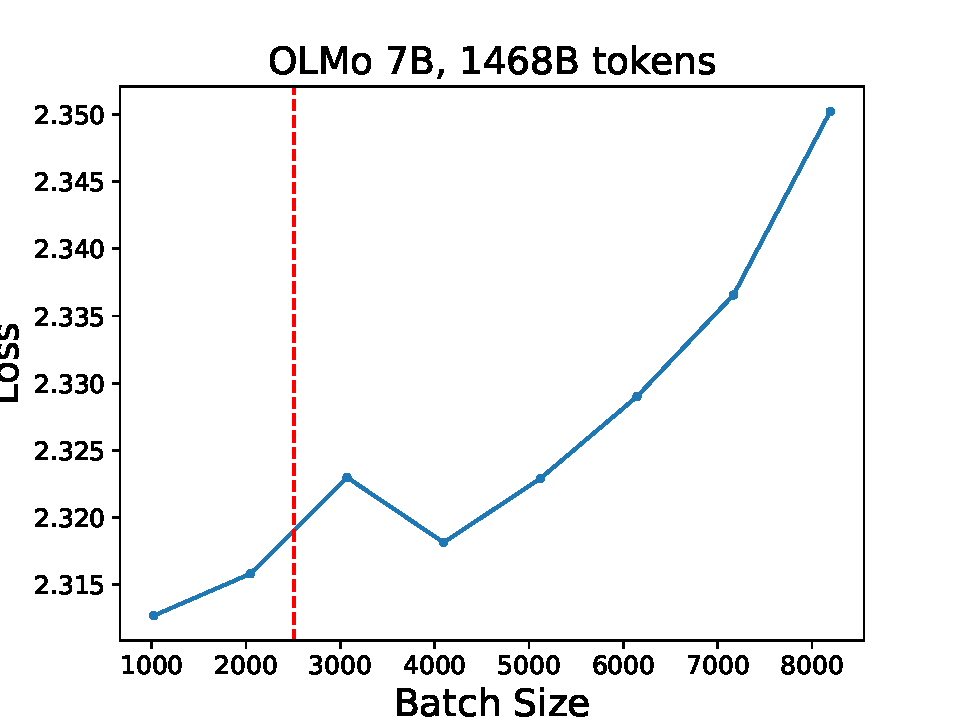
\includegraphics[width=0.32\linewidth]{figures/measure-cbs/peteish7/from350000.pdf}
    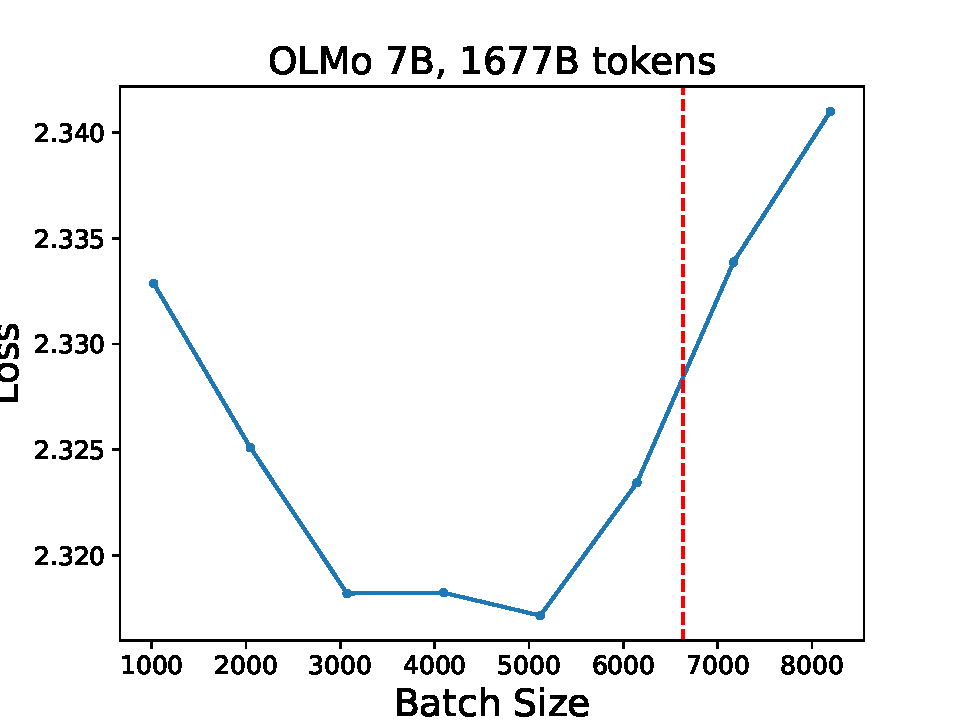
\includegraphics[width=0.32\linewidth]{figures/measure-cbs/peteish7/from400000.pdf}
    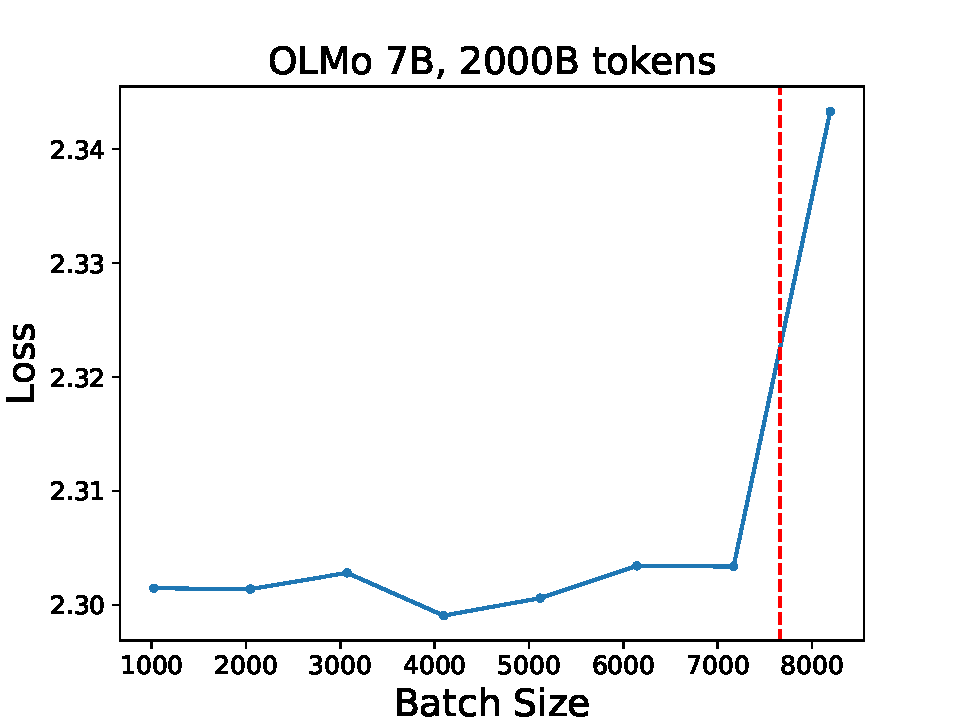
\includegraphics[width=0.32\linewidth]{figures/measure-cbs/peteish7/from477000.pdf}
    \label{fig:all-losses-7b}
\end{figure}

\section{Noise Scale Measurement Details} \label{app:noise-scale}

We use the gradient noise scale estimator proposed by \citet[Appendix A]{mccandlish2018empirical} to estimate the gradient noise scale.
The method estimates the gradient noise scale using gradient norms at two different batch sizes $\Bbig$ and $\Bsmall$ according to:
\begin{align*}
    \mathcal B_\mathrm{simple} &\approx \frac{\mathcal S}{\norm{\mathcal G}^2} , \textrm{where} \\
    \mathcal S &= \frac{\nGsmall - \nGbig}{1/\Bsmall - 1/\Bbig} \\
    \norm{\mathcal G}^2 &= \frac{\Bbig \nGbig - \Bsmall \nGsmall}{\Bbig - \Bsmall} . \\
\end{align*}
We use large batch size $\Bbig = 64$ and small batch size $\Bsmall = 1$.

It holds that $\mathbb{E} \left[ \mathcal S \right] = \mathrm{tr}(\Sigma)$ and $\mathbb{E} \left[ \norm{\mathcal G}^2 \right] = \norm{G}^2$. We thus average $\mathcal S$ and $\norm{\mathcal G}^2$ over 4096 batches reduce variance and then return their ratio as our estimate of the noise scale $\mathcal B_\mathrm{simple}$, using offline (i.e., unseen) data in each batch.

We estimate a confidence interval for $\mathcal B_\mathrm{simple}$ in two steps. First, we estimate 95\% confidence intervals for $\mathcal S$ and $\norm{\mathcal G}^2$, assuming the data are exponentially\footnote{For the exponential distribution, we use approximate confidence interval under ``Confidence Intervals'' here: \url{https://en.wikipedia.org/wiki/Exponential_distribution}.} and normally distributed, respectfully, based on manual inspection of their distributions (cf.~\Cref{fig:distributions}).
We denote these intervals $[a_{\mathcal S}, b_{\mathcal S}]$ and $[a_{\norm{\mathcal G}^2}, b_{\norm{\mathcal G}^2}]$, respectively.
We then define the confidence interval for $\mathcal B_\mathrm{simple}$ as follows:
\begin{equation*}
    \left[ \frac{a_{\mathcal S}}{b_{\norm{\mathcal G}^2}}, \frac{b_{\mathcal S}}{a_{\norm{\mathcal G}^2}} \right] .
\end{equation*}

If our estimates for $\mathcal S$ or $\norm{\mathcal G}^2$ (or their lower or upper bounds) come out negative, we consider them to be 0.

The checkpoints considered for OLMo 1B are steps 0, 10K, 20K, 40K, $\ldots$, 100K, 200K, $\ldots$ 400K.
For OLMo 7B, we use checkpoints at steps 0, 10K, $\ldots$, 40K, 60K, 70K, $\ldots$, 100K, 200K, $\ldots$ 400K.
The noise scale experiment for each checkpoint (for both the 1B and 7B models) was launched on a single GPU.

\begin{figure}
    \centering
    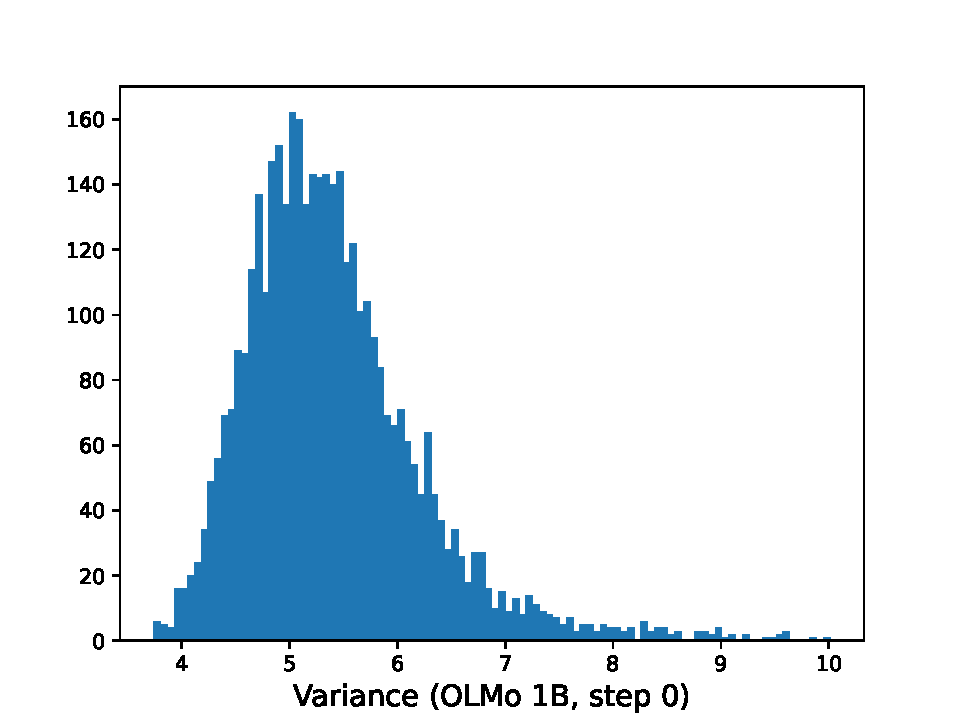
\includegraphics[width=0.48\linewidth]{figures/noise-scale/peteish1/variance.pdf}
    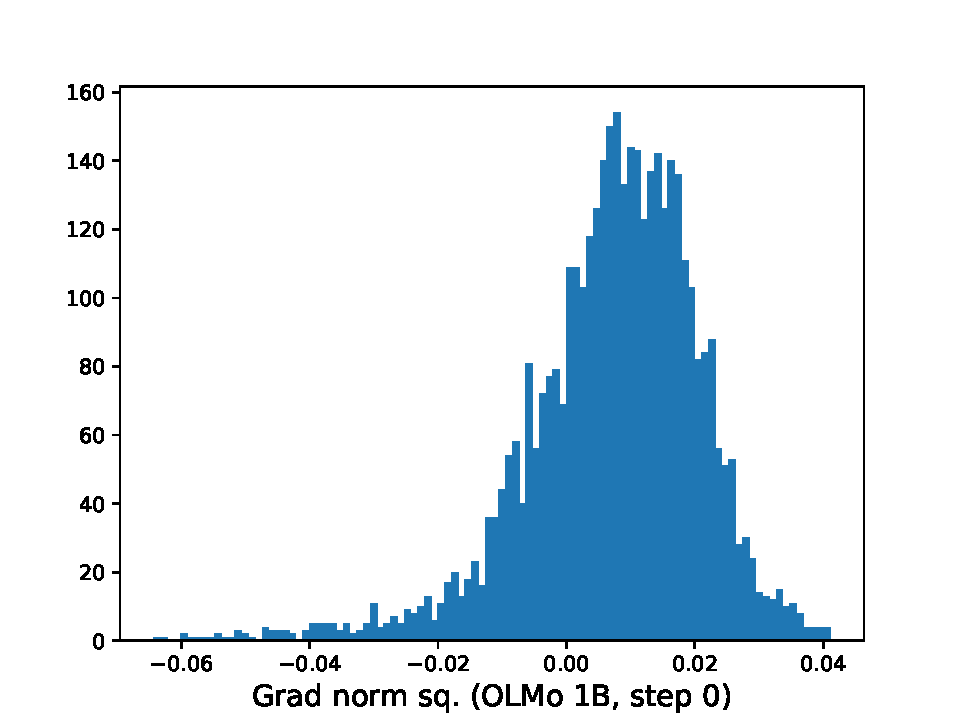
\includegraphics[width=0.48\linewidth]{figures/noise-scale/peteish1/grad-norm.pdf}
    \caption{Representative histograms for $\mathcal S$ and $\norm{\mathcal G}^2$, showing data from the 1st to 99th percentiles. The distribution for $\mathcal S$ is positive, leading us to use an exponential distribution, while the fact that some samples of $\norm{\mathcal G}^2$ are negative motivates a normal distribution.}
    \label{fig:distributions}
\end{figure}

\section{License Information} \label{sec:other-details}

The OLMo models \citep{groeneveld-etal-2024-olmo,olmo20252olmo2furious} and pretraining code, which we use, are released under Apache-2.0 license.
C4 \citep{C4} is released under ODC-BY license.
The Pile \citep{Pile} is released under MIT license.

\section{Deriving CBS Scaling Laws: An Attempt} \label{sec:scaling-laws}

In this section, we explore whether our empirical fits for the critical batch size over training can be used to derive scaling laws for aggregate critical batch size that have been derived in prior work. These scaling laws assume we want to use a fixed batch size $B$ over training, and then train many different models to the same target loss. They then measure the critical $B^*$ up to which increases in batch size do not diminish token efficiency. The standard finding from such work is that CBS grows $\propto \sqrt{T}$, where $T$ is the total training budget in tokens. This is consistent with our finding that CBS increases over the course of training---moreover, we now seek to analyze whether this scaling law can be derived from our empirical measurements of local CBS. If so, this would provide converging evidence and a simpler method for fitting CBS scaling laws that only requires training a single model.

To begin, we assume that the goal of picking a fixed batch size $B$ is to minimize the L2 distance to the local CBS over the course of training.
It is not obvious that minimizing L2 distance is the right way to pick the fixed CBS: for instance, we might want to weight training at a batch size \emph{above} the local CBS more negatively than training below it.
Regardless, we will proceed for now under the assumption that this is the right perspective.
We also make the weaker assumption that $f(t) = 0$, in line with our empirical findings (\Cref{sec:our-method}).
It follows that the best batch size to train at (i.e., fixed CBS) is simply the average local CBS over training:

\begin{restatable}{proposition}{residuals} \label{thm:residuals}
    Let $f(t)$ be integrable with $f(0) = 0$ and define
    \begin{equation*}
        R_2 = \sqrt{\int_0^T \left( B - f(t) \right)^2 \mathrm{d}t} .
    \end{equation*}
    Then $R_2$ is minimized by $B^* = \frac{1}{T} \int_0^T f(t) \mathrm{d} t$.
\end{restatable}

\begin{proof}
    We can first simplify the expression for $(R_2)^2$:
    \begin{align*}
        (R_2)^2
        &= \int_0^T \left( B - f(t) \right)^2 \mathrm{d}t \\
        &= \int_0^T \left( B^2 - 2Bf(t) + f(t)^2 \right) \mathrm{d}t \\
        &= B^2T - \int_0^T \left( 2Bf(t) - f(t)^2 \right) \mathrm{d}t .
    \end{align*}
    Now, taking the derivative with respect to $B$, we get
    \begin{equation*}
        \frac{\mathrm{d}}{\mathrm{d}B} (R_2)^2
        = 2BT - 2\int_0^T f(t) \mathrm{d} t .
    \end{equation*}
    Note that the second derivative $2T$ is positive.
    Thus, setting the derivative to $0$ and solving for $B$, we conclude that the following value of $B$ minimizes $R_2$:
    \begin{equation*}
        B = \frac{1}{T} \int_0^T f(t) \mathrm{d} t . \qedhere
    \end{equation*}
\end{proof}

% \WM{This could be generalized to even norms larger than 2 by applying the binomial expansion. To handle the 1-norm, the analysis might look a bit different.}
% \SA{This doesn't hold for any other norms. I checked 1-norm manually just to be sure.}

Thus, under the assumptions we have made, if we are trying to pick a fixed batch size that best approximates the local CBS throughout training, we can simply pick the average CBS over training.
We can use \Cref{thm:residuals} to derive a scaling law for the fixed $B^*$ as a function of the final CBS or, equivalently, the total steps $T$.
We now consider various reasonable functional forms $f(t)$ for the CBS.

\subsection{Power Law CBS Scaling}

We first consider the prediction for the fixed CBS scaling law if the local CBS evolves as a power law.

\begin{restatable}[$B^*$ for power-law CBS]{proposition}{powerlaw}
    Let $f(t) = t^c$ for $c > 0$. Then the fixed CBS is
    \begin{equation*}
        B^* = \frac{1}{c+1} T^c .
    \end{equation*}
\end{restatable}

\begin{proof}
    Plug in and solve the integral:
    \begin{align*}
        B
        &= \frac{1}{T} \int_0^T t^c \mathrm{d}t \\
        &= \frac{1}{T} \cdot \bigg[\frac{t^{c+1}}{c+1} \bigg]^T_0 \\
        &= \frac{T^c}{c+1} . \qedhere
    \end{align*}
\end{proof}

In the case where $c=1/2$ (square root), $B^* = \frac{2}{3} B^*_T = \frac{2}{3} \sqrt{T}$, which derives the $\sqrt{T}$ scaling law proposed by prior work \citep{zhang2024cbs}.

\subsection{Logarithmic CBS Scaling}

\begin{restatable}[$B^*$ for log CBS]{proposition}{logcbs}
    Let $f(t) = \log (t + 1)$. Then the fixed CBS is
    \begin{equation*}
        B^* = \frac{T}{T+1} \log (T + 1) - 1 .
    \end{equation*}
\end{restatable}

\begin{proof}
    Plug in and solve the integral:
    \begin{align*}
        B
        &= \frac{1}{T} \int_0^T \log (t + 1) \mathrm{d}t \\
        &= \frac{1}{T} \cdot \bigg[\left((t + 1) \log (t+1) - t \right) \bigg]^T_0 \\
        &= \frac{T}{T + 1} \log (T + 1) - 1 . \qedhere
    \end{align*}
\end{proof}

Thus, for large $T$, the fixed CBS will scale as $B^* \approx \log T$.

\subsection{Discussion}

These results show that, if we are choosing the fixed batch size to minimize average distance to the CBS as it evolves over training, we should pick it, more or less, as a simple function that slightly discounts the final CBS. Specifically, if we believe that the local CBS grows as $\sqrt{T}$ during training, then this derives the $\sqrt{T}$ scaling law for $B^*$ proposed in prior work.

One limitation of this view is that the L2 residuals may not be the right way to measure closeness to the CBS. In particular, it may be worse to overestimate the CBS compared to underestimate, as training above the CBS (with a scaled up learning rate) can be unstable.
We thus do not read to much into this analysis, but view it as a potentially useful starting point for future empirical and theoretical that derives CBS scaling laws from the development of the local CBS over training.

\section{BPB Evaluation on Downstream Tasks} \label{app:bpb}

This section lists the datasets we used to compute BPB measures for downstream tasks.
For multiple-choice tasks, we use the Cloze/Completion Formulation (CF), and compute the BPB metric on the gold
answer.
For completion tasks, we simply compute BPB over the correct answer.
This approach was inspired by~\citet{Bhagia2024EstablishingTS}.
The selection of tasks follows the guidelines from~\citet{DataDecide}.

\begin{table*}[t]
  \centering

    \begin{small}
    \begin{tabular}{llllll}
    \toprule
    \bf{task} & \bf{split} & \bf{\# shots} & \bf{reference}\\
    \midrule
    ARC-Challenge & Test & 5 & \citep{clark2018think} \\
    ARC-Easy & Test & 5 & \citep{clark2018think}\\
    CommonsenseQA & Val & 5 & \citep{talmor-etal-2019-commonsenseqa} \\
    HellaSwag & Val & 5 & \citep{zellers-etal-2019-hellaswag}\\
    MMLU & Val and Test & 5 & \citep{hendryckstest2021}\\
    PIQA & Val & 5 & \citep{Bisk_Zellers_Le_bras_Gao_Choi_2020}\\
    Social IQa & Val & 5 & \citep{sap-etal-2019-social}\\
    WinoGrande & Val & 5 & \citep{Sakaguchi_Le_Bras_Bhagavatula_Choi_2020}\\
    GSM8K & Gold & 5 & \citep{cobbe2021training}\\
    Minerva & Gold & 0 & \citep{lewkowycz2022solving}\\
    Humaneval & Gold & 0 & \citep{chen2021evaluating}\\
    MBPP & Gold & 0 & \citep{austin2021program}\\
    Copycolors 10-way & & 0 & \citep{Wiegreffe2024AnswerAA}\\
    \bottomrule
    \end{tabular}
    \end{small}
\end{table*}


\clearpage
%%%%%%%%%%%%%%%%%%%%%%%%%%%%%%%%%%%%%%%%%%%%%%%%%%%%%%%%%%%%

\newpage
\section*{NeurIPS Paper Checklist}

%%% BEGIN INSTRUCTIONS %%%
% The checklist is designed to encourage best practices for responsible machine learning research, addressing issues of reproducibility, transparency, research ethics, and societal impact. Do not remove the checklist: {\bf The papers not including the checklist will be desk rejected.} The checklist should follow the references and follow the (optional) supplemental material.  The checklist does NOT count towards the page
% limit. 

% Please read the checklist guidelines carefully for information on how to answer these questions. For each question in the checklist:
% \begin{itemize}
%     \item You should answer \answerYes{}, \answerNo{}, or \answerNA{}.
%     \item \answerNA{} means either that the question is Not Applicable for that particular paper or the relevant information is Not Available.
%     \item Please provide a short (1–2 sentence) justification right after your answer (even for NA). 
%    % \item {\bf The papers not including the checklist will be desk rejected.}
% \end{itemize}

% {\bf The checklist answers are an integral part of your paper submission.} They are visible to the reviewers, area chairs, senior area chairs, and ethics reviewers. You will be asked to also include it (after eventual revisions) with the final version of your paper, and its final version will be published with the paper.

% The reviewers of your paper will be asked to use the checklist as one of the factors in their evaluation. While "\answerYes{}" is generally preferable to "\answerNo{}", it is perfectly acceptable to answer "\answerNo{}" provided a proper justification is given (e.g., "error bars are not reported because it would be too computationally expensive" or "we were unable to find the license for the dataset we used"). In general, answering "\answerNo{}" or "\answerNA{}" is not grounds for rejection. While the questions are phrased in a binary way, we acknowledge that the true answer is often more nuanced, so please just use your best judgment and write a justification to elaborate. All supporting evidence can appear either in the main paper or the supplemental material, provided in appendix. If you answer \answerYes{} to a question, in the justification please point to the section(s) where related material for the question can be found.

% IMPORTANT, please:
% \begin{itemize}
%     \item {\bf Delete this instruction block, but keep the section heading ``NeurIPS paper checklist"},
%     \item  {\bf Keep the checklist subsection headings, questions/answers and guidelines below.}
%     \item {\bf Do not modify the questions and only use the provided macros for your answers}.
% \end{itemize} 
%%% END INSTRUCTIONS %%%


\begin{enumerate}

\item {\bf Claims}
    \item[] Question: Do the main claims made in the abstract and introduction accurately reflect the paper's contributions and scope?
    \item[] Answer: \answerYes{} % Replace by \answerYes{}, \answerNo{}, or \answerNA{}.
    \item[] Justification: CBS measurements in \Cref{sec:our-method} and batch size warmup tested in \Cref{sec:batch-size-warmup}.
    \item[] Guidelines:
    \begin{itemize}
        \item The answer NA means that the abstract and introduction do not include the claims made in the paper.
        \item The abstract and/or introduction should clearly state the claims made, including the contributions made in the paper and important assumptions and limitations. A No or NA answer to this question will not be perceived well by the reviewers. 
        \item The claims made should match theoretical and experimental results, and reflect how much the results can be expected to generalize to other settings. 
        \item It is fine to include aspirational goals as motivation as long as it is clear that these goals are not attained by the paper. 
    \end{itemize}

\item {\bf Limitations}
    \item[] Question: Does the paper discuss the limitations of the work performed by the authors?
    \item[] Answer: \answerYes{} % Replace by \answerYes{}, \answerNo{}, or \answerNA{}.
    \item[] Justification: Assumptions and limitations of our CBS method are discussed in \Cref{sec:our-method}.
    \item[] Guidelines:
    \begin{itemize}
        \item The answer NA means that the paper has no limitation while the answer No means that the paper has limitations, but those are not discussed in the paper. 
        \item The authors are encouraged to create a separate "Limitations" section in their paper.
        \item The paper should point out any strong assumptions and how robust the results are to violations of these assumptions (e.g., independence assumptions, noiseless settings, model well-specification, asymptotic approximations only holding locally). The authors should reflect on how these assumptions might be violated in practice and what the implications would be.
        \item The authors should reflect on the scope of the claims made, e.g., if the approach was only tested on a few datasets or with a few runs. In general, empirical results often depend on implicit assumptions, which should be articulated.
        \item The authors should reflect on the factors that influence the performance of the approach. For example, a facial recognition algorithm may perform poorly when image resolution is low or images are taken in low lighting. Or a speech-to-text system might not be used reliably to provide closed captions for online lectures because it fails to handle technical jargon.
        \item The authors should discuss the computational efficiency of the proposed algorithms and how they scale with dataset size.
        \item If applicable, the authors should discuss possible limitations of their approach to address problems of privacy and fairness.
        \item While the authors might fear that complete honesty about limitations might be used by reviewers as grounds for rejection, a worse outcome might be that reviewers discover limitations that aren't acknowledged in the paper. The authors should use their best judgment and recognize that individual actions in favor of transparency play an important role in developing norms that preserve the integrity of the community. Reviewers will be specifically instructed to not penalize honesty concerning limitations.
    \end{itemize}

\item {\bf Theory Assumptions and Proofs}
    \item[] Question: For each theoretical result, does the paper provide the full set of assumptions and a complete (and correct) proof?
    \item[] Answer: \answerYes{} % Replace by \answerYes{}, \answerNo{}, or \answerNA{}.
    \item[] Justification: Our (minor) theoretical results are fully justified in \Cref{sec:scaling-laws}.
    \item[] Guidelines:
    \begin{itemize}
        \item The answer NA means that the paper does not include theoretical results. 
        \item All the theorems, formulas, and proofs in the paper should be numbered and cross-referenced.
        \item All assumptions should be clearly stated or referenced in the statement of any theorems.
        \item The proofs can either appear in the main paper or the supplemental material, but if they appear in the supplemental material, the authors are encouraged to provide a short proof sketch to provide intuition. 
        \item Inversely, any informal proof provided in the core of the paper should be complemented by formal proofs provided in appendix or supplemental material.
        \item Theorems and Lemmas that the proof relies upon should be properly referenced. 
    \end{itemize}

    \item {\bf Experimental Result Reproducibility}
    \item[] Question: Does the paper fully disclose all the information needed to reproduce the main experimental results of the paper to the extent that it affects the main claims and/or conclusions of the paper (regardless of whether the code and data are provided or not)?
    \item[] Answer: \answerYes{} % Replace by \answerYes{}, \answerNo{}, or \answerNA{}.
    \item[] Justification: Hyperparameter information and other experimental choices are documented in \Cref{sec:cbs-measurement-details,app:noise-scale}.
    \item[] Guidelines:
    \begin{itemize}
        \item The answer NA means that the paper does not include experiments.
        \item If the paper includes experiments, a No answer to this question will not be perceived well by the reviewers: Making the paper reproducible is important, regardless of whether the code and data are provided or not.
        \item If the contribution is a dataset and/or model, the authors should describe the steps taken to make their results reproducible or verifiable. 
        \item Depending on the contribution, reproducibility can be accomplished in various ways. For example, if the contribution is a novel architecture, describing the architecture fully might suffice, or if the contribution is a specific model and empirical evaluation, it may be necessary to either make it possible for others to replicate the model with the same dataset, or provide access to the model. In general. releasing code and data is often one good way to accomplish this, but reproducibility can also be provided via detailed instructions for how to replicate the results, access to a hosted model (e.g., in the case of a large language model), releasing of a model checkpoint, or other means that are appropriate to the research performed.
        \item While NeurIPS does not require releasing code, the conference does require all submissions to provide some reasonable avenue for reproducibility, which may depend on the nature of the contribution. For example
        \begin{enumerate}
            \item If the contribution is primarily a new algorithm, the paper should make it clear how to reproduce that algorithm.
            \item If the contribution is primarily a new model architecture, the paper should describe the architecture clearly and fully.
            \item If the contribution is a new model (e.g., a large language model), then there should either be a way to access this model for reproducing the results or a way to reproduce the model (e.g., with an open-source dataset or instructions for how to construct the dataset).
            \item We recognize that reproducibility may be tricky in some cases, in which case authors are welcome to describe the particular way they provide for reproducibility. In the case of closed-source models, it may be that access to the model is limited in some way (e.g., to registered users), but it should be possible for other researchers to have some path to reproducing or verifying the results.
        \end{enumerate}
    \end{itemize}


\item {\bf Open access to data and code}
    \item[] Question: Does the paper provide open access to the data and code, with sufficient instructions to faithfully reproduce the main experimental results, as described in supplemental material?
    \item[] Answer: \answerNo{} % Replace by \answerYes{}, \answerNo{}, or \answerNA{}.
    \item[] Justification: If accepted, we will release code with the camera-ready version.
    \item[] Guidelines:
    \begin{itemize}
        \item The answer NA means that paper does not include experiments requiring code.
        \item Please see the NeurIPS code and data submission guidelines (\url{https://nips.cc/public/guides/CodeSubmissionPolicy}) for more details.
        \item While we encourage the release of code and data, we understand that this might not be possible, so “No” is an acceptable answer. Papers cannot be rejected simply for not including code, unless this is central to the contribution (e.g., for a new open-source benchmark).
        \item The instructions should contain the exact command and environment needed to run to reproduce the results. See the NeurIPS code and data submission guidelines (\url{https://nips.cc/public/guides/CodeSubmissionPolicy}) for more details.
        \item The authors should provide instructions on data access and preparation, including how to access the raw data, preprocessed data, intermediate data, and generated data, etc.
        \item The authors should provide scripts to reproduce all experimental results for the new proposed method and baselines. If only a subset of experiments are reproducible, they should state which ones are omitted from the script and why.
        \item At submission time, to preserve anonymity, the authors should release anonymized versions (if applicable).
        \item Providing as much information as possible in supplemental material (appended to the paper) is recommended, but including URLs to data and code is permitted.
    \end{itemize}


\item {\bf Experimental Setting/Details}
    \item[] Question: Does the paper specify all the training and test details (e.g., data splits, hyperparameters, how they were chosen, type of optimizer, etc.) necessary to understand the results?
    \item[] Answer: \answerYes{} % Replace by \answerYes{}, \answerNo{}, or \answerNA{}.
    \item[] Justification: Provided in \Cref{sec:cbs-measurement-details,app:noise-scale}.
    \item[] Guidelines:
    \begin{itemize}
        \item The answer NA means that the paper does not include experiments.
        \item The experimental setting should be presented in the core of the paper to a level of detail that is necessary to appreciate the results and make sense of them.
        \item The full details can be provided either with the code, in appendix, or as supplemental material.
    \end{itemize}

\item {\bf Experiment Statistical Significance}
    \item[] Question: Does the paper report error bars suitably and correctly defined or other appropriate information about the statistical significance of the experiments?
    \item[] Answer: \answerYes{} % Replace by \answerYes{}, \answerNo{}, or \answerNA{}.
    \item[] Justification: \Cref{fig:measure-cbs} shows an interval representing lower and upper bounds on the CBS, as documented in \Cref{sec:our-method}.
    \Cref{fig:noise-scale} reports a confidence interval for the noise scale whose details are documented in \Cref{app:noise-scale}.
    \item[] Guidelines:
    \begin{itemize}
        \item The answer NA means that the paper does not include experiments.
        \item The authors should answer "Yes" if the results are accompanied by error bars, confidence intervals, or statistical significance tests, at least for the experiments that support the main claims of the paper.
        \item The factors of variability that the error bars are capturing should be clearly stated (for example, train/test split, initialization, random drawing of some parameter, or overall run with given experimental conditions).
        \item The method for calculating the error bars should be explained (closed form formula, call to a library function, bootstrap, etc.)
        \item The assumptions made should be given (e.g., Normally distributed errors).
        \item It should be clear whether the error bar is the standard deviation or the standard error of the mean.
        \item It is OK to report 1-sigma error bars, but one should state it. The authors should preferably report a 2-sigma error bar than state that they have a 96\% CI, if the hypothesis of Normality of errors is not verified.
        \item For asymmetric distributions, the authors should be careful not to show in tables or figures symmetric error bars that would yield results that are out of range (e.g. negative error rates).
        \item If error bars are reported in tables or plots, The authors should explain in the text how they were calculated and reference the corresponding figures or tables in the text.
    \end{itemize}

\item {\bf Experiments Compute Resources}
    \item[] Question: For each experiment, does the paper provide sufficient information on the computer resources (type of compute workers, memory, time of execution) needed to reproduce the experiments?
    \item[] Answer: \answerYes{} % Replace by \answerYes{}, \answerNo{}, or \answerNA{}.
    \item[] Justification: Provided in \Cref{sec:cbs-measurement-details,app:noise-scale}.
    \item[] Guidelines:
    \begin{itemize}
        \item The answer NA means that the paper does not include experiments.
        \item The paper should indicate the type of compute workers CPU or GPU, internal cluster, or cloud provider, including relevant memory and storage.
        \item The paper should provide the amount of compute required for each of the individual experimental runs as well as estimate the total compute. 
        \item The paper should disclose whether the full research project required more compute than the experiments reported in the paper (e.g., preliminary or failed experiments that didn't make it into the paper). 
    \end{itemize}
    
\item {\bf Code Of Ethics}
    \item[] Question: Does the research conducted in the paper conform, in every respect, with the NeurIPS Code of Ethics \url{https://neurips.cc/public/EthicsGuidelines}?
    \item[] Answer: \answerYes{} % Replace by \answerYes{}, \answerNo{}, or \answerNA{}.
    \item[] Justification: No explanation of special circumstances necessary.
    \item[] Guidelines:
    \begin{itemize}
        \item The answer NA means that the authors have not reviewed the NeurIPS Code of Ethics.
        \item If the authors answer No, they should explain the special circumstances that require a deviation from the Code of Ethics.
        \item The authors should make sure to preserve anonymity (e.g., if there is a special consideration due to laws or regulations in their jurisdiction).
    \end{itemize}


\item {\bf Broader Impacts}
    \item[] Question: Does the paper discuss both potential positive societal impacts and negative societal impacts of the work performed?
    \item[] Answer: \answerNA{} % Replace by \answerYes{}, \answerNo{}, or \answerNA{}.
    \item[] Justification: This work is foundational research on the science of pretraining language models with no immediate impacts.
    \item[] Guidelines:
    \begin{itemize}
        \item The answer NA means that there is no societal impact of the work performed.
        \item If the authors answer NA or No, they should explain why their work has no societal impact or why the paper does not address societal impact.
        \item Examples of negative societal impacts include potential malicious or unintended uses (e.g., disinformation, generating fake profiles, surveillance), fairness considerations (e.g., deployment of technologies that could make decisions that unfairly impact specific groups), privacy considerations, and security considerations.
        \item The conference expects that many papers will be foundational research and not tied to particular applications, let alone deployments. However, if there is a direct path to any negative applications, the authors should point it out. For example, it is legitimate to point out that an improvement in the quality of generative models could be used to generate deepfakes for disinformation. On the other hand, it is not needed to point out that a generic algorithm for optimizing neural networks could enable people to train models that generate Deepfakes faster.
        \item The authors should consider possible harms that could arise when the technology is being used as intended and functioning correctly, harms that could arise when the technology is being used as intended but gives incorrect results, and harms following from (intentional or unintentional) misuse of the technology.
        \item If there are negative societal impacts, the authors could also discuss possible mitigation strategies (e.g., gated release of models, providing defenses in addition to attacks, mechanisms for monitoring misuse, mechanisms to monitor how a system learns from feedback over time, improving the efficiency and accessibility of ML).
    \end{itemize}
    
\item {\bf Safeguards}
    \item[] Question: Does the paper describe safeguards that have been put in place for responsible release of data or models that have a high risk for misuse (e.g., pretrained language models, image generators, or scraped datasets)?
    \item[] Answer: \answerNA{} % Replace by \answerYes{}, \answerNo{}, or \answerNA{}.
    \item[] Justification: No pretrained models or datasets released.
    \item[] Guidelines:
    \begin{itemize}
        \item The answer NA means that the paper poses no such risks.
        \item Released models that have a high risk for misuse or dual-use should be released with necessary safeguards to allow for controlled use of the model, for example by requiring that users adhere to usage guidelines or restrictions to access the model or implementing safety filters. 
        \item Datasets that have been scraped from the Internet could pose safety risks. The authors should describe how they avoided releasing unsafe images.
        \item We recognize that providing effective safeguards is challenging, and many papers do not require this, but we encourage authors to take this into account and make a best faith effort.
    \end{itemize}

\item {\bf Licenses for existing assets}
    \item[] Question: Are the creators or original owners of assets (e.g., code, data, models), used in the paper, properly credited and are the license and terms of use explicitly mentioned and properly respected?
    \item[] Answer: \answerYes{} % Replace by \answerYes{}, \answerNo{}, or \answerNA{}.
    \item[] Justification: The licenses for OLMo, C4, and the Pile are acknowledged in \Cref{sec:other-details}.
    \item[] Guidelines:
    \begin{itemize}
        \item The answer NA means that the paper does not use existing assets.
        \item The authors should cite the original paper that produced the code package or dataset.
        \item The authors should state which version of the asset is used and, if possible, include a URL.
        \item The name of the license (e.g., CC-BY 4.0) should be included for each asset.
        \item For scraped data from a particular source (e.g., website), the copyright and terms of service of that source should be provided.
        \item If assets are released, the license, copyright information, and terms of use in the package should be provided. For popular datasets, \url{paperswithcode.com/datasets} has curated licenses for some datasets. Their licensing guide can help determine the license of a dataset.
        \item For existing datasets that are re-packaged, both the original license and the license of the derived asset (if it has changed) should be provided.
        \item If this information is not available online, the authors are encouraged to reach out to the asset's creators.
    \end{itemize}

\item {\bf New Assets}
    \item[] Question: Are new assets introduced in the paper well documented and is the documentation provided alongside the assets?
    \item[] Answer: \answerNA{} % Replace by \answerYes{}, \answerNo{}, or \answerNA{}.
    \item[] Justification: No new assets released.
    \item[] Guidelines:
    \begin{itemize}
        \item The answer NA means that the paper does not release new assets.
        \item Researchers should communicate the details of the dataset/code/model as part of their submissions via structured templates. This includes details about training, license, limitations, etc. 
        \item The paper should discuss whether and how consent was obtained from people whose asset is used.
        \item At submission time, remember to anonymize your assets (if applicable). You can either create an anonymized URL or include an anonymized zip file.
    \end{itemize}

\item {\bf Crowdsourcing and Research with Human Subjects}
    \item[] Question: For crowdsourcing experiments and research with human subjects, does the paper include the full text of instructions given to participants and screenshots, if applicable, as well as details about compensation (if any)? 
    \item[] Answer: \answerNA{} % Replace by \answerYes{}, \answerNo{}, or \answerNA{}.
    \item[] Justification: No human subjects involved.
    \item[] Guidelines:
    \begin{itemize}
        \item The answer NA means that the paper does not involve crowdsourcing nor research with human subjects.
        \item Including this information in the supplemental material is fine, but if the main contribution of the paper involves human subjects, then as much detail as possible should be included in the main paper. 
        \item According to the NeurIPS Code of Ethics, workers involved in data collection, curation, or other labor should be paid at least the minimum wage in the country of the data collector. 
    \end{itemize}

\item {\bf Institutional Review Board (IRB) Approvals or Equivalent for Research with Human Subjects}
    \item[] Question: Does the paper describe potential risks incurred by study participants, whether such risks were disclosed to the subjects, and whether Institutional Review Board (IRB) approvals (or an equivalent approval/review based on the requirements of your country or institution) were obtained?
    \item[] Answer: \answerNA{} % Replace by \answerYes{}, \answerNo{}, or \answerNA{}.
    \item[] Justification: No human subjects involved.
    \item[] Guidelines:
    \begin{itemize}
        \item The answer NA means that the paper does not involve crowdsourcing nor research with human subjects.
        \item Depending on the country in which research is conducted, IRB approval (or equivalent) may be required for any human subjects research. If you obtained IRB approval, you should clearly state this in the paper. 
        \item We recognize that the procedures for this may vary significantly between institutions and locations, and we expect authors to adhere to the NeurIPS Code of Ethics and the guidelines for their institution. 
        \item For initial submissions, do not include any information that would break anonymity (if applicable), such as the institution conducting the review.
    \end{itemize}

\end{enumerate}

\end{document}